% TODO! list experiment, world citizenship, elite surveys, etc.
% TODO Norway and foreign aid
\clearpage
\section{Literature review}\label{sec:literature}

\subsection{Attitudes and perceptions}\label{subsec:literature_attitudes}

\subsubsection{Population attitudes on global policies}\label{subsubsec:literature_attitudes_policies}
% Our surveys fill gaps in the knowledge of attitudes toward global policies. 
% We are not aware of any other survey on a global wealth tax. 
\citet{carattini_how_2019} test the support for six variants of a global carbon tax on samples in five countries, representative along gender and age. For a given variant, the sample size is about 167 respondents per country. They find over 80\% support for any variant in India, between 50\% and 65\% in Australia, the UK and South Africa, and 43\% to 59\% in the U.S., depending on the variant. Notably, the support for a global carbon tax funding an equal dividend for each human is close to 50\% in high-income countries (e.g., at 44\% in the U.S.), consistently with our results from the \textit{Global} survey (see Figure \ref{fig:oecd}). This is another piece of evidence that the support is lower for a tax that would ``only'' reduce CO$_\text{2}$ emissions than for a quota that would unambiguously achieve the climate target. %Given that \citet{carattini_how_2019} do not explain that the policy would reduce extreme poverty and test a \textit{tax} that would only reduce CO$_\text{2}$ emissions (rather than achieve the climate target), the support is consistent with the support for a tax observed in the global survey (see Figure \ref{fig:oecd}), and somewhat lower than what the support for the GCS. 
Using a conjoint analysis in the U.S. and Germany, \citet{beiser-mcgrath_could_2019} find that the support for a carbon tax increases by up to 50\% % e.g. in their Fig. 4 the DE support for $70/t jumps from 26 to 39% with extension to all industrialized countries
if it applies to all industrialized countries rather than exclusively to one's own country. % Variant of carbon tax is 8 (US) - 17 (DE) p.p. more likely to be preferred if tax is extended to all industrialized countries

In surveys conducted in Brazil, Germany, Japan, the UK and the U.S., \citet{ghassim_who_2020} finds support ranging from 55\% to 74\% for ``a global democracy including both a global government and a global parliament, directly elected by the world population, to recommend and implement policies on global issues''. % (for example, international peace, world poverty, and climate change)''
Through an experiment, he also finds that, in countries where the government stems from a coalition, voting shares would shift by 8 (Brazil) to 12 p.p. (Germany) from parties who are said to oppose global democracy to parties that supposedly support it. For instance, when Germans respondents were told that (only) the Greens and the Left support global democracy, these parties gained respectively 9 and 3 p.p. in vote intentions, while the SPD and the CDU-CSU each lost 6 p.p. 
\citet{ghassim_who_2020} also presents survey results showing strong majorities in favor of the direct election of one's country's UN representative in all 18 surveyed countries. % same as unpa_survey_2005 % GlobeScan 2005; also: half/half (majorities or not depend on the country) for “Global Parliament, where votes are based on country population sizes, and the global parliament is able to make binding policies” (Synovate 2007); also: (GlobeScan 22, not from Ghassim) in 31 countries: 77% agree that “Rich countries must pay for poorer countries do deal with the effects of CC” 
Similarly, in each of 10 countries, there are clear majorities in favor of ``a new supranational entity [taking] enforceable global decisions in order to solve global risks'' \citep{global_challenges_foundation_attitudes_2018}. Remarkably, already in 1946, 54\% of Americans agreed (while 24\% disagreed) that ``the UN should be strengthened to make it a world government with the power to control the armed forces of all nations'' \citep{gallup_seventy_1946}. 
Furthermore, in surveys conducted in Argentina, China, India, Russia, Spain, and the U.S., \citet{ghassim_public_2022} find majority support for UN reforms that would make United Nations' decisions binding, give veto powers to a few other major countries at the Security Council, or complement the highest body of the UN with a chamber of directly elected representatives. 

Relatedly, \citet{meilland_international_2023} find that both Americans and French people prefer an international settlement of climate justice, even if it encroaches on sovereignty. In a 2013 survey conducted in China, Germany, and the U.S., \citet{schleich_citizens_2016} show that over three-quarter of people think that international climate agreements reached so far are not successful and that future agreements are important. % 73\% of people find important future international climate agreements, while less than 26\% think that international reached so far are successful. 
In Finland, \citet{sivonen_attitudes_2022} finds that that support for a carbon tax is higher if implemented at the global level (54\%) rather than at the national level (40\%).

The results from these specific questions are in line with the answers to more general questions. In each of 36 countries, \citet{issp_international_2010} find near consensus that ``for environmental problems, there should be international agreements that [their country] and other countries should be made to follow'' (overall, 82\% agree and 4\% disagree). % No question like this in the next Envi wave in 2022
In each of 29 countries, \citet{issp_international_2019} uncover near consensus that ``Present economic differences between rich and poor countries are too large'' (overall, 78\% agree and 5\% disagree). \citet{fehr_your_2022} find that only 90\% of Germans want some degree of global redistribution. %support for global and national redistribution are correlated.
%* Also in ISSP (19): slight minorities (in rich countries) that “People in wealthy countries should make an additional tax contribution to help people in poor countries.” p. 104, but strong majorities everywhere that “People from poor countries should be allowed to work in wealthy countries.” p. 106

%* ISSP (19): Near consensus that “Present economic differences between rich and poor countries are too large.” p. 102, slight minorities (in rich countries) that “People in wealthy countries should make an additional tax contribution to help people in poor countries.” p. 104, but strong majorities everywhere that “People from poor countries should be allowed to work in wealthy countries.” p. 106
%* Ghassim et al. (22): support for stronger UN with more direct elections.
%* Ghassim (20):  in Germany those two parties that supposedly endorse global democracy – the Greens and the Left – benefitted, gaining nine and three percentage points respectively in terms of voting intentions. Meanwhile, the traditional centrist parties – SPD and CDU – each lost six percentage points due to their supposed opposition to global democracy.
%* Beiser-McGrath & Bernauer (19): Conjoint analysis in US, DE. Variant of carbon tax is 8 (US) - 17 (DE) p.p. more likely to be preferred and 50% more likely to be supported if tax is extended to all industrialized countries (Fig 1, 4). (Unfortunately, don't test extension to global level).
%- Çarkoğlu.. (15) International Social Survey Program 2010 data reveal that people in LDCs are less supportive of international agreements forcing their country to take necessary environmental measures than are citizens in the developed world [80% instead of 85%]. (‘for environmental problems, there should be international agreements that [their country] and other countries should be made to follow.’)
%* Carattini et al. (Nature, 19): 1k in US, IA, ZA, AU, UK. Each respondent receives one variant at random of global carbon price of 40/60/80 $/t redistributed as international dividend / national dividend / mitigation in all countries / mitigation in developing countries / domestic mitigation / reduced labour tax. Immense majorities for any scheme in India, small majorities for each elsewhere except US international dividend (44%) or mitigation in developing (43%), and AU mitigation in developing (49,6%). PB: very low sample size (~167) for a given redistribution, even lower (~55) for a given variant (that also specifies the price). Appendix also contains estimation of distributive impacts. Representative only along the two quotas: gender and age. Don't give the representativeness in terms of income (the third socio-demos that they ask) so it's probably bad.

\subsubsection{Population attitudes on climate burden sharing}\label{subsubsec:literature_attitudes_burden_sharing}

Despite differences in the description of fairness principles, surveys on burden-sharing rules show consistent attitudes. Or at least, their seemingly contradictory results can be made compatible with the following interpretation: 
Concerning emissions reductions, most people want that every country engage in strong and collective decarbonization efforts, with a global quota converging to climate neutrality in the medium run. Concerning the financial effort, most people support high-emitting countries paying and low-income countries receiving funding. The most supported rules are those perceived as equitable, in particular an equal right to emit per person. 
% When the rankings between rules differ, it can be due to the difference in countries surveyed, but it is most often due to differences in definitions and wording. 

This interpretation helps to understand the apparent differences between articles that approach burden sharing from different angles: cost sharing (in money terms), effort sharing (in terms of emissions reductions), or resource sharing (in terms of rights to emit). Existing papers adopt either the cost sharing or effort sharing approach, which preclude any country from being a net receiver of funds. Also, by focusing on \textit{either} the financial or the decarbonization effort, these surveys miss the other half of the picture, which can explain why some papers find strong support for the ability-to-pay principle while others find strong support for grandfathering (defined as emissions reductions being the same in every country). The literature follows these approaches to align with the notions used by the UNFCCC. Yet, we argue that the resource sharing approach is preferable for uncovering attitudes, as it unambiguously describes the distributive implications of each rule while achieving an efficient geographical distribution of emissions reductions and explicitly allowing for monetary gains for some countries. % TODO? say more simply that the location of emissions reductions is flexible in resource sharing
% TODO? appendix with the definitions for each author, incl. us

Now, let us summarize the results of the different papers in the light of this clarification. 
\citet{schleich_citizens_2016} find an identical ranking of support for burden-sharing principles in China, Germany, and the U.S.: polluter-pays followed by ability-to-pay, equal emissions per capita, and grandfathering. 
% \footnote{The survey of \citet{schleich_citizens_2016} defines these rules as follows: \\
% \textit{Polluter-pays}: ``Every country has to bear costs according to the emissions it causes (hence countries causing higher emissions have a higher share of the costs).'' \\
% \textit{Ability-to-pay}: ``Every country has to bear costs according to its economic strength (hence richer countries have a higher share of the costs).''
% \textit{Egalitarianism}: ``Every country is allowed to produce the same amount of emissions per capita (hence countries with currently high emissions per capita have higher costs).''
% \textit{Sovereignty} (i.e. grandfathering): ``Every country is allowed to produce the same share of global emissions as in the past (hence the proportional reduction of emissions is the same for every country).''} 
Note that the authors do not allow for emissions trading in their description of equal \textit{emissions per capita}, which may explain its relatively low support. 
Yet, the relative support for egalitarianism also depends on how \textit{the other} rules are described. Indeed, \citet{carlsson_is_2011} find that Swedes prefer that ``all countries are allowed to emit an equal amount per capita'' rather than options where emissions are reduced based on current or historical emissions, for which it is explicitly stated that high-emitting countries ``will continue to emit more than others''. 
\citet{bechtel_mass_2013} find agreement that rich countries should pay more and historical emissions should matter, but that efforts should not be solely borne by wealthy nations. More precisely, their conjoint analysis conducted in France, Germany, the UK, and the U.S. shows that a climate agreement is 15 p.p. more likely to be preferred  (to a random alternative) if it includes 160 countries rather than 20, and 5 p.p. less likely to be preferred if ``only rich countries pay'' compared to other burden-sharing rules: ``rich countries pay more than poor'', ``countries pay proportional to current emissions'' or ``countries pay proportional to historical emissions''. %=> confirms preference for global policies (rather than only partial coverage). Finds that costs is what matters most: preference decreases by 30pp if it’s 2.5\% of GDP compared to 0.5\%.
% I have sent an email on 3/3/23 to get access to desc stats of Bechtel et al (19)
Using a choice experiment, \citet{carlsson_fair_2013} find that the least preferred option in China and the U.S. is when low-emitting countries are exempted from any effort. Ability-to-pay is appreciated in both countries and is the preferred option in the U.S., though the preferred option in China is another one that accounts for historical responsibility. %TD: it was not clear that the ability to pay was 1st in the U.S. %that Americans prefer capacity to pay > current responsibility > historical responsibility > equal emissions per capita while Chinese prefer historical > capacity > current > equal emissions.
%   Capacity to pay: Countries with high income levels must pay a larger share of the costs than countries with low income levels. This option says that countries with greater ability to pay should pay more
%   Current responsibility: Countries with currently high emissions levels must pay a larger share of the costs than countries with currently low emissions levels. This option says that those countries that are currently a larger part of the problem should pay more.
%   Historical responsibility: Countries with a history of high emissions levels must pay a larger share of the costs than countries with a history of lower emissions. This option recognizes that CO2 builds up in the atmosphere over many years. Thus, countries with a history of high emissions should pay more because they caused more of the problem.
%   Equal emissions pc: Countries with emissions per person greater than an agreed amount must pay, and they must pay more the higher their emissions per person are.
% > "equal emissions" is a misnomer as this is about costs (not emissions) and it's just a more progressive version of current responsibility / polluter-pay, where high-emitting pay more and low-emitting don't pay. The result for US is compatible with the other papers as Americans agree that rich countries (or high-emitting, the diff is small) should pay more. The Chinese position could also be reconciliable once we define responsibility from footprint rather than territorial and that there will be transfers from rich to poor countries.
In the U.S. and France, \citet{meilland_international_2023} find that the most favored fairness principle is that ``all countries commit to converge to the same average of total emissions per inhabitant, compatible with a controlled climate change''. Furthermore, in each country, 73\% disagree with grandfathering defined as ``countries which emitted a lot of carbon in the past have a right to continue emitting more than others in the future''. The study by \citet{meilland_international_2023} contains many other results: for instance, majorities prefer to hold countries accountable for their consumption-based rather than territorial emissions, and the median choice regarding historical responsibility is to hold a country accountable for its post-1990 emissions (rather than post-1850 or just their current emissions). 
% - Meilland et al. (23) find that in US and France, most favored fairness principle is Equality in per capita emissions: "all countries commit to converge to the same average of total emissions per inhabitant, compatible with a controlled climate change" and second-most (which closely follows) is grandfathering: "all countries commit to reduce their emissions by a same proportion". 73% in each disagree with grandfathering when defined as "countries which emitted a lot of carbon in the past have a right to continue emitting more than others in the future". To rationalize these contrasted views with grandfathering, we can interpret them as: equal rights, equal emission reductions, and transfers. 
%   convergence per capita (70%): all countries commit to converge to the same average of total emissions per inhabitant, compatible with a controlled climate change
%   grandfathering (60%): all countries commit to reduce their emissions by a same proportion
%   past emissions (20% choose it among their two favorite): countries which emitted less in the past commit to reduce their emissions less than other countries
%   poor countries (20%): poorer countries commit to reduce their emissions less than richer countries
%   cost-efficiency (20%): countries where reducing emissions is more costly commit to reduce their emissions less than other countries
% - Meilland et al. (23) Other findings: people prefer international settlement on CC even if it empedes on sovereignty, a majority prefers to target footprint rather than territorial emissions, median is that countries should be held accountable for post-1990 emissions, self-serving bias when judging e.g. India vs. EU, no shared understanding of fairness when asked to coordinate between French and Americans
Finally, in each of 28 (among the largest) countries, \citet{dabla-norris_public_2023} find strong majority for ``all countries'' to the question ``Which countries do you think should be paying to reduce carbon emissions?''. When asked to choose between a cost sharing based on \textit{current} vs. \textit{accumulated historic emissions}, a majority prefers \textit{current emissions} in all countries but China and Saudi Arabia (where the two options are close to equally preferred). %\hfill (Back~to~Section~\ref{subsubsec:global_support}) %In Germany and the U.S., \citet{gampfer_obtaining_2014} also find stronger support for funding climate action in low-income countries when cost is shared with other countries.

%- Gampfer (14): lab experiment (ultimatum game) to test whether preferences respect fairness principles

\subsubsection{Population attitudes on foreign aid}\label{subsubsec:literature_foreign_aid}

There is an extensive literature on attitudes towards foreign aid in donor countries. The key findings indicate that most people overestimate the amount of foreign aid and that only a minority wants a cut in foreign aid compared to actual amounts, especially once they become aware of them. 

For instance, \citet{pipa_americans_2001} shows that 83\% of Americans support a multilateral effort to cut world hunger in half. 
\citet{pipa_publics_2008} shows that in each of 20 countries, a majority thinks that developed countries ``have a moral responsibility to work to reduce hunger and severe poverty in poor countries'', with an average agreement of 81\%. In 7 OECD countries, the study finds that at least 75\% of respondents are willing to pay for a program to cut hunger in half (at an estimated cost of, e.g., \$50 a year for each American). 

\citet{kaufmann_foreign_2012} find that perceived aid is overestimated in each of the 24 countries they study, on average by a factor of 7. In most countries, desired aid is larger than perceived aid.\footnote{\citet{kaufmann_foreign_2012} offer the best results on desired aid because (as \citet{hudson_mile_2012} criticize), other studies did not take into acount misperceptions of actual aid.} They show that individuals in the top income quintile desire aid 0.13 p.p. lower than those in the bottom 40\% -- which is very close to what we find. % TODO: ref to our regression
By employing a theoretical model and examining correlations between lobbying and actual aid (controling for desired aid), they argue that the gap between actual and desired aid stems from the political influence of the rich who defend their vested interests. 
In \citet{kaufmann_foreign_2012}, the U.S. is an outlier: desired aid is at the other countries' average (3\% of GNI), but as misperceptions are enormous, perceived aid is twice as large as desired aid. Indeed, \citet{gilens_political_2001} shows that even Americans with high political knowledge misperceive actual aid, and finds that 17\% fewer of them want to cut aid when we provide them specific information about the amount of aid. % same for Hurst et al
Similarly, \citet{nair_misperceptions_2018} finds that the relatively low support for aid in the U.S. is driven by information on global distribution, as people underestimate their rank by 27 centiles on average and overestimate the global median income by a factor 10. 

\citet{hudson_mile_2012} provide a critical review of the literature and show that the strong support for poverty alleviation largely stems from intrinsic altruism. They note that, according to \citet{dfid_aid_2009} and \citet{pipa_americans_2001}, 47\% of British people find that the aid is wasted (mainly due to corruption), while Americans estimate that less than a quarter of the aid reaches those in need, with over half ending up in the hands of corrupt government officials. Despite these perceptions, most people still support aid, suggesting the presence of nonutilitarian motives. Consistent with \citet{henson_public_2010}, \citet{bauhr_does_2013} find that support for aid is reduced by the perception of corruption in recipient countries. However, this effect is mitigated by the aid-corruption paradox: countries with higher levels of corruption often need more help. %TD: `` most corrupt countries need more help.'' does not sound right to me, because ``most->more'' should be ``more->more''.
\citet{bodenstein_who_2017} further show that right-wing Europeans, as well as those who perceive strong corruption in their country, are more likely to agree that recipient countries should ``follow certain rules regarding democracy, human rights and governance as a condition for receiving EU development aid.'' 
Using a 2002 Gallup survey and the 2006 World Values Survey, and in line with \citet{bayram_aiding_2017}, \citet{paxton_individual_2012} show that the main determinants for wanting more aid are trust, left-wing ideology, interest in politics, and being a woman (all positively associated).  %\hfill (Back~to~Section~\ref{subsubsec:support_foreign_aid}) %Likewise, \citet{nair_preferences_2016} shows that preferences for international redistribution in the U.S. are netter explained by worldviews rather than socio-demographic variables. 
% heinrich_voters_2018 also show that the country's interest also play a role in aid support (as support increases when the donation can be in the country's interest) 

% Reviews, determinants
%*? Milner & Tingley (13): (highly cited but no original data, don't think we need to cite it) In 2008, 44% of American wanted foreign aid cut (american elections study, 08). fraction of federal budget going to foreign aid (mean: 27%, median: 25%) / should go (mean: 13%, median: 10%) (WorldPublicOpinion, 10)
% PIPA (01): when PIPA asked respondents to estimate how much of the federal budget was devoted to foreign aid, the median estimate was 15% -- 15 times the actual amount, which was just under 1%. More dramatically, when asked what an appropriate percentage would be, the median response was 5% -- 5 times the actual amount. And when asked to imagine that they heard the real amount was only 1%, only 18% of respondents said they thought that would be too much--as compared to the 75% who had initially said that the US was spending too much. 
%- DFID (10): Priorities: 1 NHS, 2 education, 3 support to poor countries, 4 police, 5 defence (p. 19). Show majority support for increased aid until 07, then median is to support stable aid (due to crisis?). It seems they don't give the info on actual amount though.
%* Hudson & van Heerde (12):Reviews literature on foreign aid and criticizes it on a number of points (e.g. not uncovering the determinants, and not asking well the questions). Shows strong support for poverty alleviation, (at least partly) out of intrinsic altruism. Use 4 main sources: PIPA (01, 08) UK DIDP, Eurobarometer; cf. Table 1 for all surveys on foreign aid / Public support for development has been famously described as a mile wide and and inch deep (Smillie, 1996: ref impossible to find). Hard times at home have meant that public support appears to have turned against international development efforts (Henson and Lindstrom, 2010). / Monitor public support: (Fransman and Solignac Lacomte, 2004; McDonnell et al, 2003), Paxton and Knack, 2008; Chong & Gradstein 2006. Review surveys on aid. / ~75% support aid in developed countries (stable) but ‘84 per cent agreed with the assertion that ‘taking care of problems at home is more important than giving aid to foreign countries’ (PIPA, 2001:9).” / References on covariates of aid support / PIPA 2001, "On average, Americans thought just under 25 per cent of the US budget was allocated to foreign aid, and government should allocate less than 14 per cent of the national budget. However, when told that US spends approximately 1 per cent of the federal budget on foreign aid, 37 per cent of respondents thought this was too little, 44 per cent thought it was about right, and 13 per cent thought it too much."  Think that only 23% of aid really goes to the poor / “The 2009 UK survey, Public Attitudes towards Development, reports ‘public support for overseas aid’ at 72 per cent (DFID, 2009); while in the US support was a comparable 79 per cent (PIPA, 2001); and average support across the EU trends slightly higher than in the US and UK with 91 per cent saying it was either very (53%) or fairly (38%) important to provide aid to poor countries (Eurobarometer, 2005).” / “DFID has now begun asking questions that provide relative measures of the salience of development aid vis-à-vis other competing policy issues (DFID, 2009; IDC, 2009). / "high proportion (61%) of US citizens who felt that the US spends too much on foreign aid. [from another source]” / “The distinction between foreign aid, which includes military spending, and development aid/assistance is an important one” / “81 per cent of respondents believed that developed countries do have a moral responsibility to work towards reducing hunger and severe poverty (WorldPublicOpinion.org, 2008). (…)  %/ “support for development assistance is highly contingent on respondents’ perceptions of the effectiveness of aid, especially with regard to corruption (Henson et al, 2010). For example, 
%(…) international charities and NGOs are deemed best suited/most effective compared to donor countries” / UK ‘MyAid’ plan – where the public gets to vote on how a pot of money should be distributed – / "public engagement should be about ‘opening up the political and wider societal space to the possibility of deeper change’ (Darnton and Kirk, 2011:14).”
%- Chong & Gradstein (16): from WVS 95-99, 58% want that their country give more foreign aid (but misperceptions are not taken into account)
%- Williamson (19): Public Ignorance or Elitist Jargon? Reconsidering Americans’ Overestimates of Government Waste and Foreign Aid. "Foreign aid" encompasses military spending, in the mind of American.
%- McDonnell et al (03) Public Opinion and the Fight against Poverty
%- Nair (16): preferences driven by worldviews rather than self-interest
%- Scotto et al (17): We Spend How Much? Misperceptions, Innumeracy, and Support for the Foreign Aid in the United States and Great Britain. Less American and British want aid cut when information on current aid is given in % of GDP rather than in $.
%* Paxton & Knack (12): Majorities want more aid, and main determinants are trust, ideology, interest in politics, and female (all positive). Gallup 02: in US 45% want more aid (rather than stable) vs. 68-91 in DE-UK-ES. Like Chong & Gradstein, find that desired aid increases with income, contrary to Kaufmann et al. but the latter contains more datasets.
%- Wood (15): Determinants for aid support in Australia. Wood (18) Examine Australian support for aid: although there is support to help foreign poor, people back recent aid cuts.
%- Cheng & Smyth (16): Why Give it Away When You Need it Yourself? Understanding Public Support for Foreign Aid in China. Political ideology and patriotism main explaining variables for aid support. People in poorer provinces less supportive.
%- Milner & Tingley (10) theory + empirics: who supports aid and why. owners of capital in donor countries tend to gain from aid and thus are more likely to support giving aid
%- Easterly (JEP, 03) Can Foreign Aid Buy Growth? No (disproves Hansen & Tarp).
%- Hansen & Tarp (01) Aid increases growth (empirical evidence)
%- Tresch et al. (22): 66% of Swiss people want to increase their foreign aid; also Borofsky
%- Harris (17): majority of French want to decrease foreign aid when face with a trade-off with other public spending

\subsubsection{Population attitudes on rich tax}\label{subsubsec:literature_wealth_tax}

We are not aware of any previous survey on a global wealth tax,\footnote{We did not find any using the combination of ``survey'' or ``attitudes'' with ``wealth tax'' or ``global wealth tax'' in Google Scholar.} though surveys consistently show strong support for national wealth taxes. 
In a comprehensive survey conducted in the UK, \citet{rowlingson_public_2021} show that a wealth tax is the preferred option for raising revenues. Only 8\% of respondents state that total net wealth should not be taxed (with little differences between Labour and Conservative voters). The study also finds that the preferred design would be a 1\% or 3\% tax on net wealth above £1 million. 
By asking how much taxes per year should a person with a certain income and wealth level pay, \citet{fisman_americans_2017} finds that the average American favors a 0.8\% linear tax rate on unspecified wealth up to \$2 million (the highest wealth level tested), and a 3\% linear rate on inherited wealth. %This is consistent with the findings of \citet{chirvi_preferences_2020}. 
Through a conjoint analysis conducted in three high-income countries, \citet{schechtl_tax_2023} find widespread support for a wealth tax (from 78\% in the U.S. to 86\% in Germany and the UK), with a preference for an exemption threshold set at \$/\euro{}1 million (rather than 500,000 or 2 million) with the tax rate and tax unit having little influence on the preferred design. 
In 21 OECD countries, the \citet{oecd_main_2019} uncovers strong majority support for higher taxes on the rich to support the poor, with nearly 70\% overall agreement and less than 20\% disagreement. \citet{isbell_footing_2022} finds similarly high level of support in 34 African countries. 
In the UK, \citet{patriotic_millionaires_patriotic_2022} find 69\% support (and 7\% opposition) for a 1.1\% tax on wealth in excess of £10 million. 
In the U.S., \citet{americans_for_tax_fairness_support_2021} find that 67\% to 71\% of the respondents support to ``raise taxes for those earning more than \$400,000 a year'', ``raise the income tax rate for those earning over \$1 million a year by 10 percentage points'', or ``apply a 2\% tax on an individual's wealth above \$50 million each year, and 3\% on wealth above \$1 billion''.
%- Gallup (22), US
%- Fight Inequality Alliance India (22), IA

% PIPA (01): what percentage of their "tax dollars that go to help poor people at home and abroad...should go to help poor people in other countries." The mean response was 16% (down a bit from 22% in response to this question in a 1996 PIPA poll). Strikingly, this turns out to be a far higher percentage than is currently given. In 1999, a bit less than 4% of the total spent on the poor went to the poor abroad. Sixty percent of respondents proposed a percentage that was higher than 4%.

% TODO! list experiment

\subsubsection{Population attitudes on ethical norms}\label{subsubsec:literature_wealth_tax}
% \paragraph{World citizenship}

\paragraph{Universalism}
% No need to cite: Buntaine & Prather (18), Diederich & Goeschl (18) Willingness to act for domestic vs. international climate action
Various studies have examined the concept of global identity (see %e.g. \citet{mcfarland_all_2012}, or 
\citet{reysen_psychology_2018} for a review). In the 2005-2008 wave of the World Values Survey, \citet{bayram_what_2015} notes that ``78\% of the participants in 57 countries see themselves as citizens of the world'', though the \href{https://www.worldvaluessurvey.org/WVSDocumentationWV7.jsp}{2017-2022 wave} reveals that more people feel close to their town, region or country than to the world. \citet{enke_universalism_2023} measure universalism at the U.S. district level using donation data, and find that a district's universalism predicts electoral outcomes better than its income or education level. To measure universalism at the individual level, \citet{enke_moral_2023-1} ask American respondents to split \$100 between a random stranger and a random person with the same income but closer to them. They distinguish different facets of universalism, and define \textit{foreign universalism} as the inclination to give to a foreigner rather than a fellow citizen. They find a home bias for most people, which could partly be attributed to concerns about inequality, as the split involves two persons with the same income, with the foreigner most certainly living in a poorer country than the American and thus enjoying a higher social status. 
That being said, a home bias probably remains even after accounting for concerns about  inequality, as 84\% of Americans agree that ``taking care of problems at home is more important than giving aid to foreign countries'' \citep{pipa_americans_2001}. 
\citet{enke_moral_2023} also measure universalism and analyze its correlates in 7 countries, and \citet{cappelen_universalism_2022} deploy this method in 60 countries. 
In a lab experiment with students in the U.S., \citet{cherry_accepting_2017} show that a substantial share of people prefer policies detrimental to them due to their egalitarian worldview. \citet{waytz_ideological_2019} show that left-leaning people exhibit a wider ``moral circle''. \citet{jaeger_relative_2021} find that judgments of moral concern are equally well explained by characteristics of the judge and the evaluated target.
% Evidence that people are altruistic: they experience higher temperature when they learn they are doing good (Taufik et al. 15), they are sensitive to self-transcending more than self-interested reasons (Evans et al. 13), 

\paragraph{Free-riding}

Despite the long-standing explanation of the lack of climate action as a result of free-riding, surveys consistently show that people support climate mitigation action in their own country, even in the absence of such action in other countries. \citet{bernauer_how_2015} show this for Americans and Indians, who both overestimate their country's emissions at one third of the global total. \citet{beiser-mcgrath_commitment_2019} show this in the U.S. and China using an experimental design. \citet{mcevoy_prospects_2016} show that Americans mostly invoke leadership and morality to justify unilateral climate action. Using a range of methods, \citet{aklin_prisoners_2020} show that the empirical evidence for free-riding is not compelling, and that climate inaction can be equally well explained by distributive conflicts. Finally, review of the literature by \citet{mcgrath_how_2017} shows that climate attitudes are largely nonreciprocal, and primarily driven by values and perceptions of the policies, rather than by considerations of what other countries do.

\subsubsection{Second-order beliefs}\label{subsubsec:literature_beliefs}

\citet{allport_social_1924} introduced the concept of pluralistic ignorance: a shared misperception concerning others' beliefs. The concept became notorious when \citet{ogorman_pluralistic_1975} showed that, towards the end of the civil rights movement, 47\% of Americans believed that a majority of white people supported segregation, while only 18\% did so. %\citet{miller_pluralistic_1987} shows that pluralistic ignorance emerges because individuals believe that fear of embarrassment is a sufficient cause for their own behavior but not for the behavior of others. 
\citet{pipa_americans_2001} has shown that while 75\% of Americans are willing to contribute \$50 annually to halve world hunger (the cost of the program), only 32\% believed that the majority would share this willingness. 
Pluralistic ignorance regarding climate-friendly norms in the United States has been documented by \citet{andre_fighting_2021}. Similarly, \citet{sparkman_americans_2022} show that Americans underestimate the support for climate policies by nearly half, while \citet{drews_biased_2022} document pluralistic ignorance of carbon tax support in Spain. 
Additionally, \citet{geiger_climate_2016} show that pluralistic ignorance regarding concern for climate change leads people to self-silence, resulting in reduced discussions on the topic.
% TODO READ Mildenberg & Tingley (19) and improve summary
%- Bursztyn & Yang (21): Review of the field. Misperceptions about others are widespread, asymmetric, much larger when about out-group members, and positively associated with one’s own attitudes.
%* Andre et al. (21): Respondents vastly underestimate the prevalence of climate- friendly behaviors and norms among their fellow citizens. Providing respondents with correct information causally raises individual willingness to fight climate change as well as individual support for climate policies. The effects are strongest for individuals who are skeptical about the existence and threat of global warming.
%- Di Tella et al. (AER, 15): The results of the lab experiment favor the hypothesis that people avoid altruistic actions by distorting beliefs about others' altruism
%- Allport (1924): first book on pluralistic ignorance
%- Allport (40): function of poll is to correct pluralistic ignorance
%- Studies on pluralistic ignorance: business (Buckley et al. 00), against affirmative action (Van Boven 00), political correctness (Braghieri, AER 21), alcohol (Suls & Green, 03), white support for racial segregation (O'Gorman 75), CC (Geiger & Swim 16), hooking up (Lambert et al 03, cf. note for paragraph of pluralistic ignorance), women working outside home in Saudi Arabia (Bursztyn et al. 20)
% Leviston et al. (2013 in: Drews et al., 2022, p. 2) found that people overestimated the proportion of people being climate sceptic,

% \subsubsection{Elite attitudes}\label{subsubsec:literature_beliefs} % TODO!

% \citet{mildenberger_beliefs_2019} survey elites (Congress staffers and international relations scholars) as well as the population in U.S. and China. They document pluralistic ignorance of pro-climate attitudes, egocentric bias, and increasing support after beliefs are updated. 
% \citet{lange_importance_2007} \citet{lange_self-interested_2010}
% \citet{dannenberg_equity_2010}
% \citet{kesternich_negotiating_2021} 
% \citet{hjerpe_common_2011}

% Elite surveys 
%* Mildenberg & Tingley (19): Congress staffers, cf. second-order beliefs
%- Hertel-Fernandez et al. (2019): Survey on US Congress staffers (not on climate)
%- Milner & Tingley (10) (not sure it's a survey) owners of capital in donor countries tend to gain from aid and thus are more likely to support giving aid
%- Lange et al. (Energy Econ, 2007): climate negotiators.  Mix of self-serving bias and support for egalitarian principle.
%- Lange et al. (EER, 2010): same data as Lange et al. (10)
%- Dannenberg et al. (ERE, 2010): elicit climate negotiators’ equity preferences using Fehr & Schmidt (99) method => regional differences in addressing climate change are driven more by national interests than by different equity concerns
%- Kesternich et al. (EEPS, 2020): survey on climate negotiators about their preferred burden-sharing rules: we observe tendencies for a more harmonized view among key groups towards the ability-to-pay rule in a setting of weighted burden sharing rules
%- Lange & Schwirplies (ERE, 2017): combines Lange et al. (10) and Schleich et al.
%* Hjerpe et al. (2011): Delegates at COP2009. The results indicate that voluntary contribution, indicated as willingness to contribute, was the least preferred principle among both negotiators and observers. Three of the four principles for allocating mitigation commitments were recognized widely across the major geographical regions: historic 1990, capacity to pay, and equal per capita emissions. The difference was never below 25 percentage units, and the opponent share never exceeded 16%.
%- Scholte et al. (2020)
%- Bayram (17): cosmopolitanism of German politicians and their respect of international law

\subsection{Proposals and analyses of global policy-making}\label{subsec:literature_policies}

\subsubsection{Global carbon pricing}\label{subsubsec:literature_pricing}

Global carbon pricing is widely regarded by economists as the benchmark climate policy, as it would efficiently correct the carbon emissions externality. For instance, \citet{hoel_carbon_1991} shows that an international carbon tax can be designed to simultaneously achieve efficiency and accommodate any distributional objective. 
Concerning the distributional objective, \citet{grubb_greenhouse_1990}, \citet{agarwal_global_1991} and \citet{bertram_tradeable_1992} were the first to advocate for an equal right to emit for each human. As \citet{grubb_greenhouse_1990} states it: ``by far the best combination of long term effectiveness, feasibility, equity, and simplicity, is obtained from a system based upon tradable permits for carbon emissions which are allocated on an adult per capita basis''.\footnote{By ``adult per capita'', \citet{grubb_greenhouse_1990} means that permits would be allocated equally among adults.} Support for such solution has been renewed ever since \citep{baer_equity_2000,jamieson_climate_2001,blanchard_major_2021,rajan_global_2021}. %TD: je ne comprends pas le terme ``adult per capita'', je suis surpris par la formule (adult/capita, ??), je pensais que c'était une typo. Je suppose que c'est une tournure standar dqui m'échappe.

While many endorse the egalitarian allocation of emissions permits, economists also considered this outcome as politically unfeasible. Thus, to preserve the current level of inequalities and to preclude transfers between countries, they adjusted their (integrated assessment) models by assigning more weight to the interest of rich countries \citep{stanton_negishi_2011}.  %As a result, they have adjusted their (integrated assessment) models by assigning more weight to rich countries' interests to preserve the current level of inequalities between countries, precluding any transfer between them \citep{stanton_negishi_2011}. 

\citet{gollier_negotiating_2015} synthesize the distributional decision with a \textit{generosity} parameter which would allocate emissions permit to countries in proportion to their population if set to one, in proportion to their emissions (on the start date of the policy) if set to zero, and as a mixture of the egalitarian and grandfathering rules if set in between. Using a similar formula in the context of a tax, \citet{cramton_international_2015} (summarized in \citealp{mackay_price_2015}) propose that countries with emissions per capita around the average fix the generosity parameter, so that it is strategically chosen to maximize the tax rate, and to fix the tax rate at the minimum price proposed by participating countries. Negotiations would exclude countries with low ambition beforehand; and the treaty would impose trade sanctions on non-participating countries. %  In \citet{cramton_global_2017}, prominent economists discuss how such negotiations can succeed, and whether a tax or tradable quotas has better chances. The tax is recommended in most chapters (except in the one of Gollier \& Tirole)
\citet{bergh_dual-track_2020} propose a ``dual-track transition to global carbon pricing'': an expanding climate club that would integrate existing and new emissions trading systems, and a reorientation of UNFCCC negotiations towards a global carbon price and burden-sharing rules. 
The \citet{imf_how_2019} also supports global carbon pricing or, as a first step, a carbon price floor. They propose either differentiated prices among countries or international transfers, and estimate that a price of \$75/tCO$_\text{2}$ in 2030 would be compatible with a 2\textdegree{}C trajectory. %Similarly, \citet{parry_proposal_2021} acknowledges that transfers could be necessary to induce climate action in low- and middle-income countries, though they mention transferring only 1\% of carbon revenues. 

Other authors have put forth more radical proposals. For instance, \citet{weitzman_world_2017} envisions a World Climate Assembly with proportional representation at the global scale, so that the median (human) voter would choose the carbon price level. % and each country retaining the revenues TODO?
To finance an adaptation fund, \citet{chancel_carbon_2015} propose a global \textit{progressive} carbon tax (or a progressive tax on air tickets as a first step), so that rich people (who are high emitters) contribute more to the public good. 
\citet{fleurbaey_climate_2013} highlight that, given that current emitters are probably richer than future victims of climate change damages, climate policies deserve a \textit{negative} discount rate. In other words, we cannot dissociate the climate issue from global inequalities, and an ethical response to this issue requires global redistribution. 
%* Cramton et al (17): Livre de pontes. Tout le monde est d'accord : un prix mondial du carbone est requis, il ne peut être obtenu que par la réciprocité des engagements (style climate club), et il faut quelques transferts des riches vers les pauvres ainsi que des sanctions commerciales pour aligner les incitations. Ch 4 (also Cramton et al 15) propose la formule suivante de transfert (positif ou négatif) à un fonds climat : générosité*émissions en excès (par rapport à la cible)*prix du carbone. Le livre argumente bcp sur prix vs. quantité (TLM préfère prix sauf Gollier & Tirole), l'argument le plus convaincant en faveur du prix c'est qu'avec la procédure proposée le prix négocié serait le plus élevé possible, alors qu'avec la quantité c'est le budget carbone qui serait le point focal et ça aboutirait à une impasse (objectif trop ambitieux). 
%* Weitzman (17) advocates for a World Climate Assembly, choosing the price level with the median voter, and each country retaining the revenues.
% Fleurbaey & Zuber (13): The discount rate converges to the worst-off (affected by the measure) to the worst-off (beneficiary of the measure) discount rate, which depends on the growth between both agents. Applied to real data, we can consider that the worst-off affected by a global tax on CO_2 is the average-earner on earth (around 75% centile i.e. ~1000€/month, cf. Chancel & Piketty, Lakner & Milanovic, Chakravorty) while the worst-off beneficiary is the worst-off person in the future (among those less affected by CC thanks to the measure), probably below 1000€/month => negative discount rate.
% Parry et al (21): Proposal for an International Carbon Price Floor Among Large Emitters. Acknowledges that transfers could be necessary to induce climate action in low/middle-income countries, talks about transferring 1% of carbon revenues.
%- Sager: distributive effects of global pricing without int'l transfers.
%- Budolfson et al. (incl. Fleurbaey, Méjean, Zuber, Dennig) (21): global carbon price with within-country per capita dividend. Acknowledge that "The overall benefits to society are even greater if total carbon tax revenues are returned on an equal per capita basis globally, which directs more of the revenues towards the poorest populations in the world (rather than the poorest within each country or region)." Very short (3p, no appendix, no suppl. info)
%- Chancel & Piketty (15): global progressive carbon tax
% Pottier et al (17): A survey of global climate justice 

\subsubsection{Climate burden sharing}\label{subsubsec:literature_burden_sharing} 

The literature has discussed different burden-sharing principles. While there is no  agreement on their definitions as different approaches are used (cost sharing, effort sharing, or resource sharing, see Section \ref{subsubsec:literature_attitudes_burden_sharing}), we describe here the burden-sharing principles consistently using the resource sharing approach (i.e., allocating emissions rights). 

\paragraph{Equal per capita.} The simplest principle is perhaps to allocate each year's global carbon quota based on an equal right to emit per capita, or an equal right to emit for each adult. Implementing this principle would result in large transfers from high-emitting to low-emitting countries. 

\paragraph{Grandfathering.} In contrast, \textit{grandfathering} entails allocating emissions rights in proportion to current emissions. From the perspective of allocating carbon pricing revenues between countries, grandfathering amounts to each country retaining the revenues it collects. Given that nations are sovereign and have not agreed to share emissions rights, this principle can be considered as the default option against which the other ones can be compared in terms of distributive effects.

\paragraph{Historical responsibilities.} At the opposite end of the spectrum is the principle of \textit{historical responsibilities}, which assigns to each country a carbon budget proportional to its population. Countries that have emitted more than the average have accumulated a carbon debt towards countries that have emitted less, which have a carbon credit.\footnote{It is not clear how these debts would be settled. Approaches could involve carbon removal from the atmosphere, or using a conventional social cost of carbon to monetize them, by crediting (positively or negatively) emissions rights to countries in an international carbon market.} 

To fully specify this rule, one needs to define a start date for the responsibilities on past emissions and specify how to account for population size. 1990 is often chosen as a start year as it is the date of the first IPCC assessment report, marking the widespread acknowledgment of climate change, though variants include 1972, 1960, 1950 or 1850.\footnote{\href{https://climateequitymonitor.in}{Climate equity monitor} uses 1850 for example.} Several solutions have been proposed to account for evolving populations, none of which is flawless. \citet{matthews_quantifying_2015} allocates emissions rights on a given year proportionally to the countries' populations in that year. An alternative is to use fixed populations, such as the populations at the chosen start year \citep{neumayer_defence_2000}, or at a future date such as projected when the global total population will reach 9 billion \citep{raupach_sharing_2014}. \citet{fanning_compensation_2023} convert the projected climate debt up to 2050 into monetary terms in a 1.5\textdegree{}C scenario.% (using the average of 2020--2050 marginal abatement costs as the carbon price).

The rationale for using fixed populations is to prevent countries from intentionally increasing their population size to gain more emissions rights. However, this approach treats countries with different demographic trajectories similarly, effectively penalizing countries which grow more than others (if past populations are used) or grow more than expected (if future populations are used). Using current populations like \citet{matthews_quantifying_2015} also comes with its own problems. Consider two countries having contributed very little to cumulative emissions, with the same emissions per capita but different demographic patterns: country A's population has doubled in the last 30 years, while country B's population has remained stable. Despite the similar present situation, country B would accumulate more carbon credit than country A. Essentially, compensating country B more due to its past population size amounts to compensating the dead although it is future generations who will suffer. That being said, using current populations is likely a more viable solution than relying on fixed populations since, in practice, countries with similar emissions per capita tend to have relatively similar demographic trajectories.

\paragraph{Ability to pay.} Another prominent burden-sharing principle is the ability to pay whereby richer countries should contribute more to mitigation efforts. To operationalize this principle, \citet{baer_greenhouse_2008} define \textit{capacity} as the share of global income above an exemption threshold. They use the threshold of \$7,500 per year (in 2005 PPP), which corresponds to the top 28\% of the global income distribution. According to this principle, the effort of a country should be proportional to the revenues it would raise with a linear income tax on individual income above \$7,500. 

% \paragraph{Greenhouse Development Rights.} 
\paragraph{Climate Equity Reference Framework} \citet{baer_greenhouse_2008} %actually 
propose another effort-sharing method, %originally 
%dubbed the \textit{greenhouse development rights} (GDR)
%but now renamed 
the \textit{Climate Equity Reference Framework} (CERF), which blends the ability to pay principle with their version of historical responsibilities. They define \textit{responsibility} as follows: they determine the mitigation requirement as the emissions gap between the Business as Usual scenario from \citet{iea_world_2007} and a 2\textdegree{}C (with 68-86\% probability) scenario. The mitigation requirement is then allocated to countries proportionally to their cumulative emissions (starting in 1990). The emissions right of a country according to their \textit{responsibility} are then determined by its Business as Usual emissions minus its mitigation requirement. A country's emissions right, dubbed its \textit{greenhouse development right} (GDR), 
%The GDR of a country 
is defined using a combination of \textit{capacity} (C) and \textit{responsibility} (R) to allocate the mitigation requirement between countries. This allocation key is called the \textit{Responsibility and Capacity Indicator} (RCI) and defined as $RCI = R^{a}\cdot C^{1-a}$, with $a=.4$. % TODO! canonical article is Holz et al 18

This choice of parameter may seem somewhat arbitrary, but the \href{https://climateequityreference.org}{EcoEquity calculator} allows for a customization all CERF %GDR 
parameters \citep{holz_climate_2019}. The Climate Action Network has adopted the CERF %GDR 
as its \textit{fair share} framework, though the different national chapters of the organization could not agree on a choice of parameters \citep{athanasiou_fair_2022}.% This paper is one of the best to read in this subsection
\footnote{The \href{https://usfairshare.org/}{U.S. Climate Action Network} and the think tank \href{https://www.ecoequity.org/about/}{EcoEquity} (funded by Tom Athanasiou and late Paul Baer) choose the following parameters: an equal weight for R and C ($a=.5$), their own \href{https://climateequityreference.org/calculator-information/gdp-and-emissions-baselines/}{business as usual projections} of CO$_\text{2}$ emissions based on trends of GDP growth and emissions intensity reduction,  % Given all this, our strategy is a modest one. As we mention above and explain in greater detail below, our algorithm for projecting CO2 emissions is based on combining estimates of emissions intensity reduction with estimates of GDP growth, with the values for both derived from a convergence from historical rates of change to projected long-term (through 2030) rates of change. To limit the influence of climate policies, we have elected to utilize the rates of change for GDP and emissions intensity from a set of baseline scenarios that are included in the scenario database of the IPCC’s Fifth Assessment report (the baseline scenarios of the EMF27 modelling exercise, to be precise)
a 1.5\textdegree{}C (Low Energy Demand) pathway, 1950 as the start year for responsibility, a gradual inclusion of income to compute \textit{capacity} (which adds complexity to the calculation) from a full exemption of the bottom 70\% (\$7,500 per year) linearly to a full inclusion of the top 2\% (\$72,211), the inclusion of non-CO$_\text{2}$ gases but not of emissions embodied in trade (i.e. imported emissions) nor LULUCF (land-use). }

\begin{figure}[h!]
    \caption[Net gains with the CERF burden-sharing rule.]{Net gains from the CERF burden-sharing rule in 2030. }\label{fig:gain_gdr_over_gdp_2030}
    \makebox[\textwidth][c]{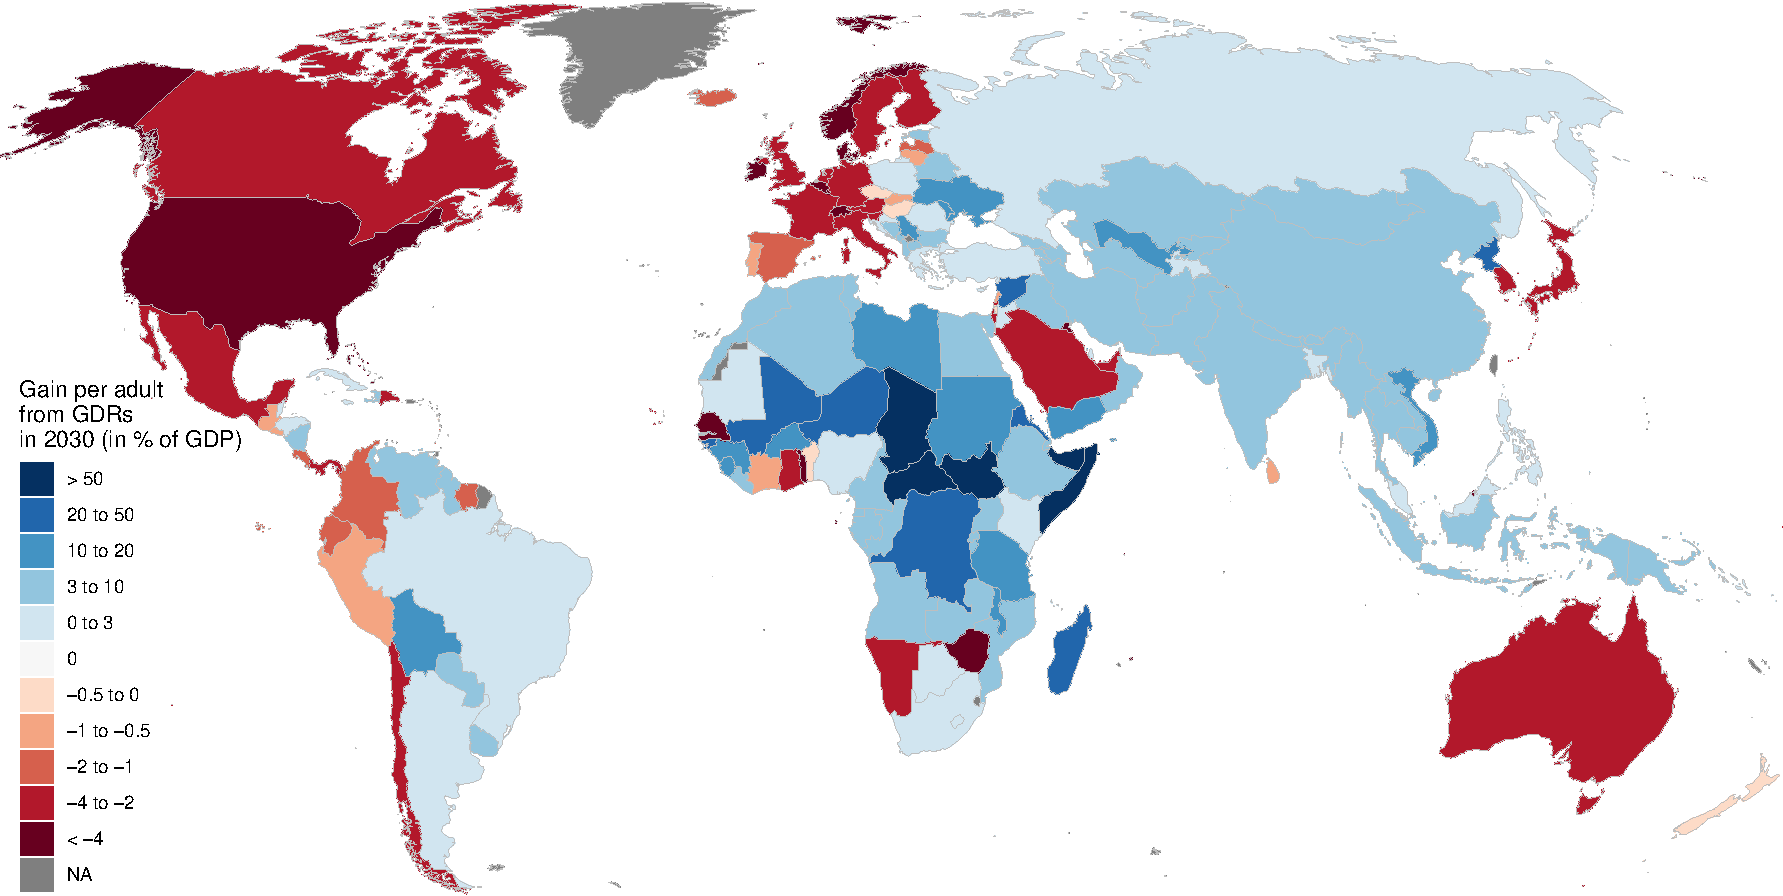
\includegraphics[width=\textwidth]{../figures/maps/gain_gdr_over_gdp_2030.pdf}} 
    {\small \textit{Note:} GDRs are calibrated with the preferred parameters of the \href{https://usfairshare.org/}{U.S. Climate Action Network} \citep{athanasiou_fair_2022} using the Efficiency scenario (2\textdegree{}C with $>$50\% chance) of the Global Energy Assessment \citep{johansson_global_2012} and a price of \$144/tCO$_\text{2}$.}
\end{figure} 

\begin{figure}[h!]
    \caption[Comparison between GDR and equal per capita burden-sharing rules.]{Difference between net gains from Greenhouse Development Rights and equal rights per capita. }\label{fig:diff_gain_gdr_gcs_over_gdp_2030}
    \makebox[\textwidth][c]{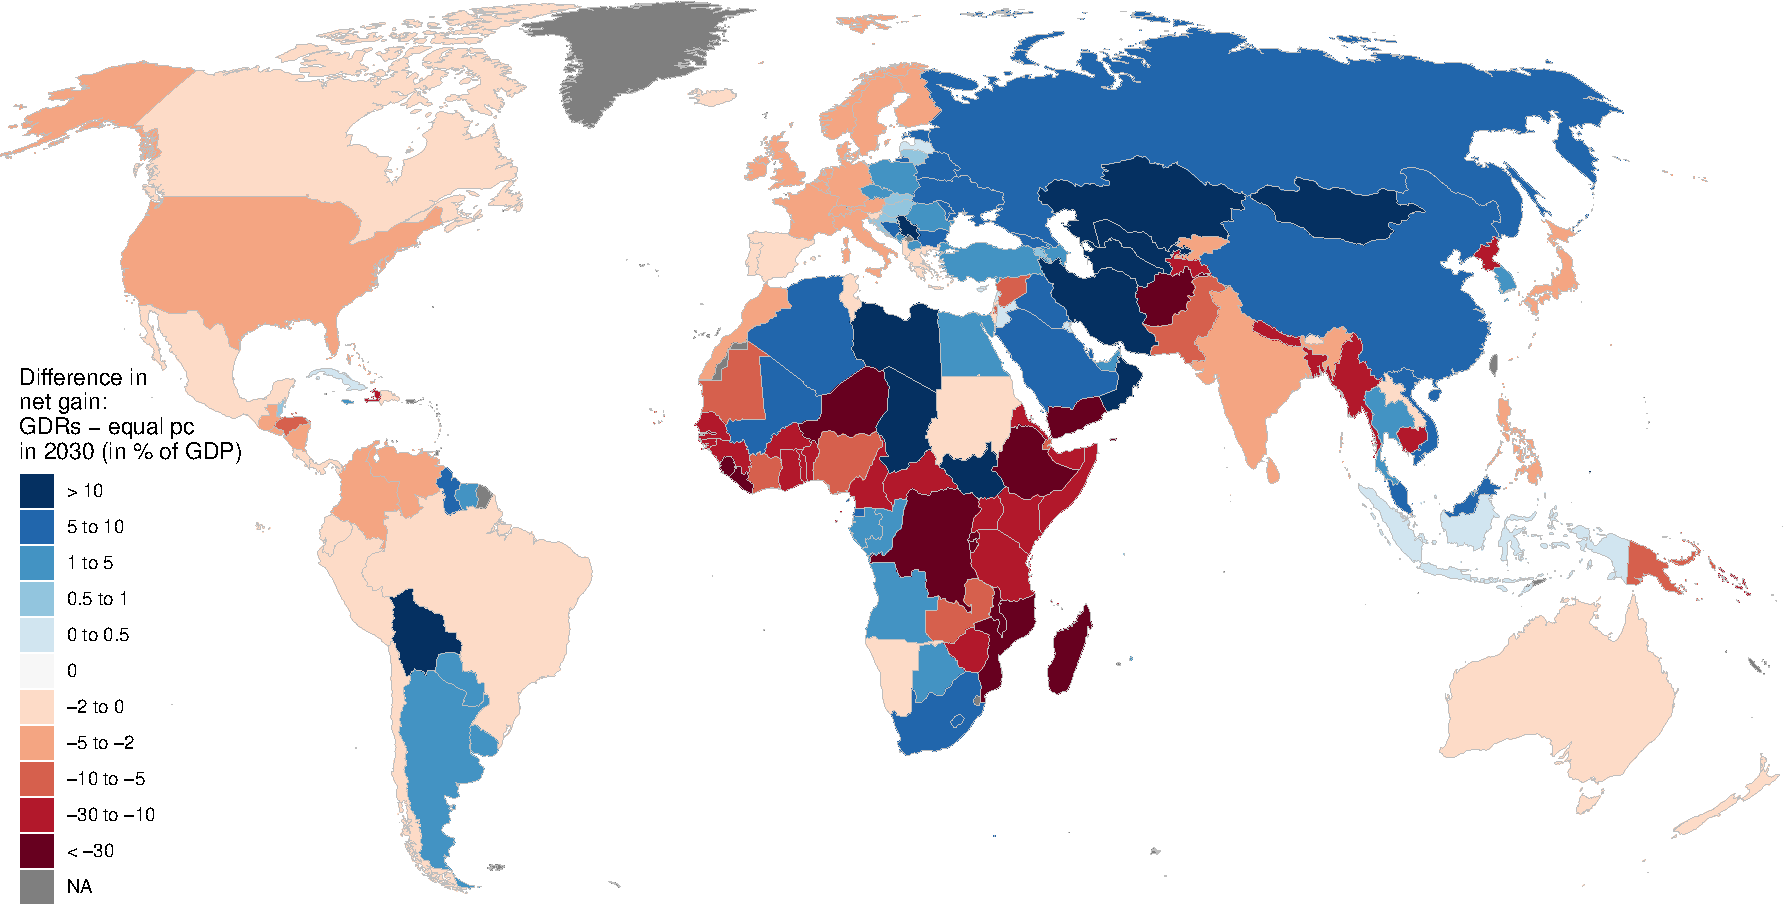
\includegraphics[width=\textwidth]{../figures/maps/diff_gain_gdr_gcs_over_gdp_2030.pdf}} 
    {\small \textit{Note:} GDRs are calibrated with the preferred parameters of the \href{https://usfairshare.org/}{U.S. Climate Action Network} \citep{athanasiou_fair_2022} using the Efficiency scenario (2\textdegree{}C with $>$50\% chance) of the Global Energy Assessment \citep{johansson_global_2012} and a price of \$144/tCO$_\text{2}$.}
\end{figure} % TODO? GDR -> CERF in figure?

The CERF %GDR 
approach was adopted by a prominent network of climate NGOs because it operationalizes the principle of \textit{common but differentiated responsibilities and respective capabilities} recognized by the UNFCCC. However, this approach suffers from three drawbacks. %important limitations. 
First, its definition of historical responsibility as an effort sharing principle is inconsistent with the principle of an equal right of cumulative emissions per capita, which is a resource sharing principle. For instance, consider a fully decarbonized country that has exhausted \textit{exactly} its cumulative carbon budget. According to the CERF notion of \textit{responsibility}, this country would still be expected to contribute significantly to mitigation efforts due to its relatively high cumulative emissions. Yet, according to the usual definition of the historical responsibility based on an equal right of cumulative emissions p.c., this country would have no liability as it has not exceeded its carbon budget. 
Second, a country with moderate incomes\footnote{Using the above parameters, moderate incomes means few incomes above the global 70th. percentile.} and low historical responsibility would be assigned a relatively low effort, even if its emissions per capita are high. In other words, the CERF %GDR 
approach favors countries that have experienced recent growth. % , like China
Third, the poorest countries would be granted emissions rights close to the Business as Usual trajectory, as they would bear virtually none of the effort. But this trajectory carries the current (unfair) income distribution and amounts to grandfathering. For example, the baseline trajectory for emissions\footnote{The baseline trajectory is computed as the ``product of the projected GDP and CO$_\text{2}$ emission intensity''.} in the DRC entail 0.8 tCO$_\text{2}$ p.c. in 2030, %(this is 16\% more than in 2020, but a lot lower than the global objective of about 4t). 
which is five times less than the world average emissions right per capita. In this framework, if the DRC were to grow faster than projected in the baseline, it would actually have to pay to the rest of the world for mitigation efforts. This is what is likely to happen to countries like Mexico or Senegal, from our simulation of the net gains of CERF compared to a situation without international transfers (see Figure \ref{fig:gain_gdr_over_gdp_2030}). 
In contrast, a resource sharing approach based on equal per capita emissions would result in low-income countries receiving emissions rights exceeding their projected trajectories, leading to transfers from high-income countries. By construction, such transfers do not occur in an effort sharing approach like the CERF, implying lower transfers to low-income countries. %GDR. 
Compared to an equal right to emit per capita, this method favors countries like China (whose emissions are allowed to remain stable over 2020-2030 instead of a reduction of 35-40\%) and penalizes regions like Sub-Saharan Africa and Latin America (see Figure \ref{fig:diff_gain_gdr_gcs_over_gdp_2030}). 

\paragraph{Contraction and Convergence.} \citet{meyer_briefing_2004} defines a rule called \textit{contraction and convergence} (C\&C), which combines elements of grandfathering and equal per capita approaches. According to C\&C, each country is granted (tradable) emissions rights, starting at their current emission level and converging linearly to an equal per capita level at some pre-specified date. The \textit{contraction} part refers to the reduction of total emissions rights in line with the climate objective. When discussed around year 2000, the convergence date was specified between 2020 and 2050. This rule, advocated by the Global Commons Institute (a UK think tank), was on the agenda from COP2 to COP15 (i.e., until Copenhagen, and including in Kyoto), including at Kyoto, and was endorsed by the European Parliament in 1998. More recently, \citet{gignac_allocating_2015} have shown how C\&C can be made consistent with historical responsibilities by computing carbon debts and credits until the convergence date.

\paragraph{Assessments of the NDCs against burden-sharing principles.} 
The regime established by the 2015 Paris agreement to regulate climate change respects none of the burden-sharing principles and relies instead on voluntary contributions from each country, known as Nationally Determined Contributions (NDCs). A body of literature (reviewed by \citealp{hohne_regional_2014}) assesses the NDCs against the emissions reduction objective and different burden-sharing principles. To evaluate the NDCs, \citet{gao_sufficient_2019} examine their emissions projections for 2030 and estimate the resulting increase in temperature. The most recent and comprehensive assessment of NDCs against burden-sharing principles is conducted by \citet{van_den_berg_implications_2020} (see also \citealp{robiou_du_pont_national_2016,robiou_du_pont_equitable_2017,raupach_sharing_2014}). 

%- Riahi et al. (17), Bauer et al. (17), Van Vuuren et al. (SSP1, 17), Kriegler et al. (SSP5, 16), Fricko et al (SSP2, 17): SSPs => Is SSP5 compatible with RCP2.6? Apparently, according to Riahi not really (Fig. 8) but it still appears in Bauer (Fig. 2) and Yes, according to Kriegler et al (17)
% Scenarios with low emissions:
% - SSP1/2/5-2.6 (or -1.9). (RCP1.9: 1.4°C en 2100 -> 1°C 2300 / 2.6: 1.8 °C -> 1.5 / 4.5: 2.7°C -> 3.3 https://global-climat.com/2021/09/02/rapport-ar6-du-giec-le-point-sur-la-temperature-globale/)
% - Global Energy Assessment (Johansson 12), e.g. Efficiency scenario
% - Greenpeace [Advanced] [R]evolution (Teske 15) 
% - NDCs (Gao et al 19). Check difference SSP2-4.5 with NDCs in 2030. Extend the NDCs either with SSP2 or with some assumption e.g. convergence to SSP2-2.6.
% - Decent Living: Kikstra et al 21
% - Low Energy Demand (Grubler): only has Global North and South
% - IEA ETP17 2DS and B2DS: doesn't have Africa nor GDP nor population
%- https://climateequitymonitor.in/ computes carbon debt based on equal per capita cumulative emissions. contact@climateequitymonitor.in https://twitter.com/equity4climate

% money/CO2 need to meet decent living standards: Kistra et al 21, Hallegatte et al 23 (TODO: read), Millward-Hopkins et al 20, Bruckner et al 22

\subsubsection{Global redistribution}\label{subsubsec:literature_redistribution}
% TODO? Give a stat on income disparities between countries?
% SDG, need for int'l transfers
Addressing global poverty, inequalities, and climate change are central to the universally agreed Sustainable Development Goals (SDG). % 12 out of  17
As highlighted by \citet{bolch_arithmetics_2022}, low-income countries often lack sufficient domestic resources to eradicate poverty in the short term, indicating the need for international transfers to rapidly end global poverty. %In other words, it would hardly be possible to achieve the first SDG and end extreme poverty by 2030 without international transfers. % Zhang (16) estimates the poverty gap in each country. Global one is at $80G/year.
%This shows that international transfers would be needed to rapidly end global poverty. 
%The lack of solidarity from high-income countries has been long criticized. 
In \textit{Beyond the Welfare State}, Gunnar \citet{myrdal_beyond_1960} called for a \textit{welfare world}. In his Nobel lecture, he emphasized the necessity of increasing foreign aid to low-income countries, stating that ``The type of marginal foreign aid we have provided, is clearly not enough to meet their barest needs'' \citep{myrdal_equality_1975}.

% Unequal exchange, Hickel
Drawing on the labor theory of value, some economists have argued that global inequalities arise from unequal exchange in international trade \citep{arghiri_unequal_1972}. Indeed, the stark disparity in wages between countries implies that one unit of labor exported by an American commands five units of labor embodied in imported goods, whereas Ethiopians need to export 50 units of labor to obtain one unit through imports \citep{alsamawi_employment_2014,reyes_better_2017}.
Taking stock, \citet{hickel_divide_2017} proposes to globally establish minimum wages at 50\% of the local median wage. \citet{hickel_divide_2017} also suggests other solutions against global inequality, which served as inspiration for our questionnaire. These measures include the cancellation of low-income countries' public debt, fair trade practices (such as eliminating tariffs from high-income countries, reducing patent protections, and reducing farming subsidies in rich countries), initiatives to combat tax evasion (e.g., implementing a global financial register), land reform, and a fair international climate policy. 

\citet{piketty_capital_2014} prominently advocates for a progressive wealth tax on a global scale, although he does not specify whether the resulting revenues should fund international transfers. %how the revenues should be used, nor whether there should fund international transfers.% and it was implicit that each country would retain the revenues it collected. 

% Unfairness of current tax rates
\citet{kopczuk_limitations_2005} compute the optimal linear income tax rates for all countries in two ways: globally centralized and decentralized (i.e., within each country and without international transfers). They show that the average decentralized rate is 41\%. In contrast, the global rate is 62\%, which would generate funds to finance a basic income of 250\$/month (higher than the GPD per capita of 73 countries). From a current global Gini index of 0.695, they show that decentralized optimal taxation would only marginally reduce global inequality to 0.69, whereas global taxation would significantly decrease the Gini to 0.25. The study also shows that the existing level of foreign aid can only be rationalized if the U.S. attaches 2,000 less value to a citizen in the poorest countries than to an American citizen (or 1,000 less if half of the transfers are diverted due to corruption). 

% Carthy & Walsh (Oxfam, 22) propose various sources of funding for damages.
% Piketty (2014) "At what rate would [a global wealth tax] be levied? One might imagine a rate of 0 percent for net assets below 1 million euros, 1 percent between 1 and 5 million, and 2 percent above 5 million. Or one might prefer a much more steeply progressive tax on the largest fortunes (for example, a rate of 5 or 10 percent on assets above 1 billion euros). There might also be advantages to having a minimal rate on modest-to-average wealth (for example, 0.1 percent below 200,000 euros and 0.5 percent between 200,000 and 1 million)" He doesn't explicitly talk about revenue use, but implicitly they would be retained by each collecting country: "Le rôle principal de l'impôt sur le capital n'est pas de financer l'État social, mais de réguler le capitalisme.", "En principe, chaque pays de l'Union européenne pourrait obtenir des recettes du même ordre en appliquant seul un tel système."

\subsubsection{Basic income}\label{subsubsec:literature_basic_income}

Unconditional cash transfers (UCT) are increasingly seen as an effective way to end extreme poverty. A growing body of evidence from randomized control trials supports this notion: \citet{gangopadhyay_cash_2015} find that UCT outperform a food subsidy; \citet{haushofer_short-term_2016} find significant impacts on health, economic outcomes, and psychological well-being; \citet{egger_general_2022} find large positive spillovers on non-recipient people, and minimal inflation. 
Reviews of existing research further confirm the positive outcomes of UCT \citep{standing_little_2014,bastagli_cash_2016}. % TD: from the Cambridge dictionary, ``extant'' is ``used to refer to something very old that is still existing''', so I think ``existing'' fits better. Same comment applies to other occurrences of ``extant''.

While the delivery of cash to remote areas and the prevention of fraud is challenging in regions without a proper civil register, the use of mobile phones as banking and biometric identification tools could provide viable solutions \citep{harnett_taking_2017}. Although many places still lack internet access, satellite internet technology shows promising progress, with some experts suggesting that it could soon become affordable and universally accessible \citep{hanson_satellite_2016}.

\subsubsection{Global democracy}\label{subsubsec:literature_democracy}

The idea of world federalism has a long-standing history, dating back at least to \citet{kant_zum_1795}, who argued that a world federation was essential for achieving perpetual peace. 
International organizations were eventually created to foster peace, though the League of Nations and its successor, the United Nations, never succeeded in avoiding military conflicts. 
Many have argued that we need stronger and more democratic global institutions, competent to address global challenges such as extreme poverty, climate change, wars, pandemics, or financial stability. 
Before World War II, feminist and pacifist \citet{maverick_lloyd_chaos_1937} founded the \textit{Campaign for World Government}, advocating for direct representation at the global scale. 
\citet{einstein_general_1947} called for the subordination of the UN Security Council to the General Assembly and the direct election of UN delegates. 
Since 2007, there has been widespread support for a United Nations Parliamentary Assembly (UNPA) from individuals and institutions in over 150 countries, including 1,800 member of parliament, heads of state, as well the European Parliament, the Pan-African Parliament, and the Latin-American Parliament. The UNPA campaign calls for a gradual implementation of a democratic assembly, starting with a consultative assembly composed of members of national parliaments, allowing for the direct election of its members in voluntary countries, and progressing towards a world parliament with binding legislative powers once all members are directly elected \citep{leinen_world_2018}. % READ Ch 13, 21, 22, 26
Besides the UNPA, various scholars have put forward different models of global democracy, ranging from deliberative spaces to a world federation \citep{archibugi_global_2011}. % TODO READ and expand, also read marchetti_global_2008
%Using surveys covering 86\% of global population, \citet{hale_could_2019} find that the world as a whole is less polarized that some countries and argue against the fear people's views would be too diverse for a functioning global democracy. 
While the most radical proposals may still be on the horizon, an assembly of random citizens representative of the world population has already been convened. It has produced a joint statement at the COP26 \citep{global_assembly_report_2022}, and a similar \textit{World Citizens' Assembly} should soon follow. 
% Stanford dico (kuyper_global_2016)? 

% ___________________________

% Burden-sharing
%- Agarwal & Narain (91) first to defend an equal right to emit per capita (equal to the absorbing capacity of the Earth)
%- Gampfer (14): lab experiment (ultimatum game) to test whether preferences respect fairness principles
%- Chancel & Piketty (15): global progressive carbon tax
% cf. bottom

% Global policies attitudes 
%* ISSP (19): Near consensus that “Present economic differences between rich and poor countries are too large.” p. 102, slight minorities (in rich countries) that “People in wealthy countries should make an additional tax contribution to help people in poor countries.” p. 104, but strong majorities everywhere that “People from poor countries should be allowed to work in wealthy countries.” p. 106
%* Ghassim et al. (22): support for stronger UN with more direct elections.
%* Ghassim (20):  in Germany those two parties that supposedly endorse global democracy – the Greens and the Left – benefitted, gaining nine and three percentage points respectively in terms of voting intentions. Meanwhile, the traditional centrist parties – SPD and CDU – each lost six percentage points due to their supposed opposition to global democracy.
%* Beiser-McGrath & Bernauer (19): Conjoint analysis in US, DE. Variant of carbon tax is 8 (US) - 17 (DE) p.p. more likely to be preferred and 50% more likely to be supported if tax is extended to all industrialized countries (Fig 1, 4). (Unfortunately, don't test extension to global level).
%- Çarkoğlu.. (15) International Social Survey Program 2010 data reveal that people in LDCs are less supportive of international agreements forcing their country to take necessary environmental measures than are citizens in the developed world [80% instead of 85%]. (‘for environmental problems, there should be international agreements that [their country] and other countries should be made to follow.’)
%* Carattini et al. (Nature, 19): 1k in US, IA, ZA, AU, UK. Each respondent receives one variant at random of global carbon price of 40/60/80 $/t redistributed as international dividend / national dividend / mitigation in all countries / mitigation in developing countries / domestic mitigation / reduced labour tax. Immense majorities for any scheme in India, small majorities for each elsewhere except US international dividend (44%) or mitigation in developing (43%), and AU mitigation in developing (49,6%). PB: very low sample size (~167) for a given redistribution, even lower (~55) for a given variant (that also specifies the price). Appendix also contains estimation of distributive impacts. Representative only along the two quotas: gender and age. Don't give the representativeness in terms of income (the third socio-demos that they ask) so it's probably bad.


% Global policies
%* Beyond the welfare state: Myrdal 58
% Pottier et al (17): A survey of global climate justice 
%* Hickel (17): The Divide: A Brief Guide to Global Inequality and its Solutions
%* Kopczuk et al (EER, 17) Compute optimal linear tax rate for all countries in two ways: decentralized or globally. Shows that the tax rate increases with inequality of skills (calibrated with the gini). The average decentralized rate is 0.41 The global one 0.62, with a global demogrant of 250$/month (higher than 73 countries' GDP). Show that within decentralized/country optimal taxation would not decrease global inequality by much (gini from 0.695 to 0.69, but down to 0.25 with global income tax). Show that USA don't give a damn of poor countries' people. citizens in the US (one of the richest) attach only 1/(2,000\*a) of the weight to the welfare of citizens in poorest countries, where a is the share  of transfer (supposedly) effectively arriving to the recipients. e.g. if half of aid is wasted by corrupt politicians, the weight is 1/1000.
% Carthy & Walsh (Oxfam, 22) propose various sources of funding for damages.
% Piketty (2014) "At what rate would [a global wealth tax] be levied? One might imagine a rate of 0 percent for net assets below 1 million euros, 1 percent between 1 and 5 million, and 2 percent above 5 million. Or one might prefer a much more steeply progressive tax on the largest fortunes (for example, a rate of 5 or 10 percent on assets above 1 billion euros). There might also be advantages to having a minimal rate on modest-to-average wealth (for example, 0.1 percent below 200,000 euros and 0.5 percent between 200,000 and 1 million)" He doesn't explicitly talk about revenue use, but implicitly they would be retained by each collecting country: "Le rôle principal de l'impôt sur le capital n'est pas de financer l'État social, mais de réguler le capitalisme.", "En principe, chaque pays de l'Union européenne pourrait obtenir des recettes du même ordre en appliquant seul un tel système."

% Global carbon pricing TODO find current advocates of GCS
%* Grubb (90), Betram (92) advocate for global market with equal pc right
%* Bergh et al. (20) call for a "dual-track transition to global carbon pricing": an expanding climate club, and "a reorientation of UNFCCC negotiations creates room for talking seriously about a global carbon price schedule, including redistribution-of-revenues rules." They don't specify which equity rules to use.
%* Jamieson (01) advocates of equal pc burden-sharing (after the precursors Agarwal & Narain (91))
%* Bear et al (Science, 00), Bear (02), Athanasiou & Baer (02) advocate for equal pc burden-sharing (although weirdly, Bear & Athanasiou then change mind and advocate for the Greenhouse Development Rights, accounting for capacity and responsibility)
%* Cramton et al (17): Livre de pontes. Tout le monde est d'accord : un prix mondial du carbone est requis, il ne peut être obtenu que par la réciprocité des engagements (style climate club), et il faut quelques transferts des riches vers les pauvres ainsi que des sanctions commerciales pour aligner les incitations. Ch 4 (also Cramton et al 15) propose la formule suivante de transfert (positif ou négatif) à un fonds climat : générosité*émissions en excès (par rapport à la cible)*prix du carbone. On demanderait aux États autour de la moyenne d'émission de fixer ce paramètre de générosité, pour qu'il soit fixé de sorte à maximiser le prix, puis on fixerait le prix comme le prix minimum proposé (après avoir éjecté qqs pays récalcitrants des négos). Puis, sanctions commerciales pour ceux qui ne respectent pas le prix. Ch Gollier & Tirole proposent une formule aussi simple que l'autre : quota global*((1-g)*part des émissions à t=0 + g*part de la population), où g joue le même rôle de paramètre de générosité/éthique (que je voudrais mettre à 1, mais qu'ils disent tous de mettre < 1 pour que les pays riches acceptent. Le livre argumente bcp sur prix vs. quantité (TLM préfère prix sauf Gollier & Tirole), l'argument le plus convaincant en faveur du prix c'est qu'avec la procédure proposée le prix négocié serait le plus élevé possible, alors qu'avec la quantité c'est le budget carbone qui serait le point focal et ça aboutirait à une impasse (objectif trop ambitieux).
% Blanchard & Tirole
%* MacKay et al (Nature, 15) summarizes the above
%* Weitzman (17) advocates for a World Climate Assembly, choosing the price level with the median voter, and each country retaining the revenues.
% Fleurbaey & Zuber (13): The discount rate converges to the worst-off (affected by the measure) to the worst-off (beneficiary of the measure) discount rate, which depends on the growth between both agents. Applied to real data, we can consider that the worst-off affected by a global tax on CO_2 is the average-earner on earth (around 75% centile i.e. ~1000€/month, cf. Chancel & Piketty, Lakner & Milanovic, Chakravorty) while the worst-off beneficiary is the worst-off person in the future (among those less affected by CC thanks to the measure), probably below 1000€/month => negative discount rate.
% Stanton (11): Negishi weights obviate the IAMs’ equalization of income. 4 ways to solve this problem: 1. be more transparent, 2. stop weighting, 3. take linear utility (i.e. maximize global GDP), 4. stop optimizing. 
% Hoel (91): Shows that an international tax can be designed so that it is both efficient and satisfies whatever distributional objectives one might have.
% IMF (2019): global pricing (with either differentiated prices or international transfers) or, as a first step, a carbon price floor. 25% of revenues should be rebated to the bottom 40%, the rest used to reduce distortionary taxes or for green investments. Estimate that $75/t is needed in 2030 for 2°C.
% Parry et al (21): Proposal for an International Carbon Price Floor Among Large Emitters. Acknowledges that transfers could be necessary to induce climate action in low/middle-income countries, talks about transferring 1% of carbon revenues.
%- Sager: distributive effects of global pricing without int'l transfers.
%- Budolfson et al. (incl. Fleurbaey, Méjean, Zuber, Dennig) (21): global carbon price with within-country per capita dividend. Acknowledge that "The overall benefits to society are even greater if total carbon tax revenues are returned on an equal per capita basis globally, which directs more of the revenues towards the poorest populations in the world (rather than the poorest within each country or region)." Very short (3p, no appendix, no suppl. info)

% Foreign aid 
%* Kaufmann et al (12) Shows the level of perceived and desired aid in 26 countries between 2005 and 2008 (cf. Table 1). In most countries (incl. UK, DE, FR, ES but not U.S.) desired aid is larger than perceived. Argue that this is due to political influence efforts/possibilities of the rich, as they prefer less aid due to vested interests (support this by a theoretical model + correlations between level of lobbying and actual aid level, controling for desired aid). In most countries the gap between the two is small, except in the U.S. where perceived is 7.5% of GDP and preferred is 3%.Use WVS and Gallup (like Chong & Gradstein, Paxton & Knack) but have more waves and the others don't use the question on perceived aid. Shows that richer want less aid ("those in the top income quintile favour ODA (as a share of GNI) that is 0.13 percentage points lower than the preferred share for individuals in the bottom 40\% of the income distribution" after controling for perceived aid - our regression results are sensibly the same.). from 0 to higher than 25%: threshold at 0.05; 0.15; 0.35; 0.75; 1.5; 2.5; 4; 7.5; 17.5; 25, i.e. same number of thresholds but small than ours below 2.5 and higher above. 
%*? Milner & Tingley (13): (highly cited but no original data, don't think we need to cite it) In 2008, 44% of American wanted foreign aid cut (american elections study, 08). fraction of federal budget going to foreign aid (mean: 27%, median: 25%) / should go (mean: 13%, median: 10%) (WorldPublicOpinion, 10)
% PIPA (01): Overwhelming majorities support a multilateral effort to cut hunger in half by the year 2015 and say that they would be willing to pay for the costs of such a program. However, most do not think that the average American would be as willing to pay the necessary costs. when PIPA asked respondents to estimate how much of the federal budget was devoted to foreign aid, the median estimate was 15% -- 15 times the actual amount, which was just under 1%. More dramatically, when asked what an appropriate percentage would be, the median response was 5% -- 5 times the actual amount. And when asked to imagine that they heard the real amount was only 1%, only 18% of respondents said they thought that would be too much--as compared to the 75% who had initially said that the US was spending too much. what percentage of their "tax dollars that go to help poor people at home and abroad...should go to help poor people in other countries." The mean response was 16% (down a bit from 22% in response to this question in a 1996 PIPA poll). Strikingly, this turns out to be a far higher percentage than is currently given. In 1999, a bit less than 4% of the total spent on the poor went to the poor abroad. Sixty percent of respondents proposed a percentage that was higher than 4%.
%- DFID (10): Priorities: 1 NHS, 2 education, 3 support to poor countries, 4 police, 5 defence (p. 19). Show majority support for increased aid until 07, then median is to support stable aid (due to crisis?). It seems they don't give the info on actual amount though.
%* PIPA (08): Across 20 countries, 81% support that "developed countries have a moral responsibility to help reduce hunger ansevere poverty in poor countries (majority in every country). “the World Bank (Shantayanan et al, 2002) has estimated that it will require an extra US$39-54 billion per year to meet Millennium Development Goal 1 (MDG1). (…) The per person cost of meeting MDG1 came to £25 for the UK, $56 for the US, €27 for Germany, and so on. On average 77 per cent of respondents are in favour of contributing towards meeting the goal (provided that all others do too). To take the US example, 75 per cent of people supported paying an extra $56 per year to meet MDG1. What is significant about this figure is that it is only slightly below the support for the ‘cost free’ question as to whether the US should be willing to share a  small portion of its wealth with those who are in great need (79%).” Hudson & van Heerde (12)
%* Hudson & van Heerde (12):Reviews literature on foreign aid and criticizes it on a number of points (e.g. not uncovering the determinants, and not asking well the questions). Shows strong support for poverty alleviation, (at least partly) out of intrinsic altruism. Use 4 main sources: PIPA (01, 08) UK DIDP, Eurobarometer; cf. Table 1 for all surveys on foreign aid / Public support for development has been famously described as a mile wide and and inch deep (Smillie, 1996: ref impossible to find). Hard times at home have meant that public support appears to have turned against international development efforts (Henson and Lindstrom, 2010). / Monitor public support: (Fransman and Solignac Lacomte, 2004; McDonnell et al, 2003), Paxton and Knack, 2008; Chong & Gradstein 2006. Review surveys on aid. / ~75% support aid in developed countries (stable) but ‘84 per cent agreed with the assertion that ‘taking care of problems at home is more important than giving aid to foreign countries’ (PIPA, 2001:9).” / References on covariates of aid support / PIPA 2001, "On average, Americans thought just under 25 per cent of the US budget was allocated to foreign aid, and government should allocate less than 14 per cent of the national budget. However, when told that US spends approximately 1 per cent of the federal budget on foreign aid, 37 per cent of respondents thought this was too little, 44 per cent thought it was about right, and 13 per cent thought it too much."  Think that only 23% of aid really goes to the poor / “The 2009 UK survey, Public Attitudes towards Development, reports ‘public support for overseas aid’ at 72 per cent (DFID, 2009); while in the US support was a comparable 79 per cent (PIPA, 2001); and average support across the EU trends slightly higher than in the US and UK with 91 per cent saying it was either very (53%) or fairly (38%) important to provide aid to poor countries (Eurobarometer, 2005).” / “DFID has now begun asking questions that provide relative measures of the salience of development aid vis-à-vis other competing policy issues (DFID, 2009; IDC, 2009). / "high proportion (61%) of US citizens who felt that the US spends too much on foreign aid. [from another source]” / “The distinction between foreign aid, which includes military spending, and development aid/assistance is an important one” / “81 per cent of respondents believed that developed countries do have a moral responsibility to work towards reducing hunger and severe poverty (WorldPublicOpinion.org, 2008). (…) there are a good number of people who support aid despite the fact they do not think it works. What this suggests – but cannot show in any detail – is that people have nonutilitarian motives for supporting aid.” / “support for development assistance is highly contingent on respondents’ perceptions of the effectiveness of aid, especially with regard to corruption (Henson et al, 2010). For example, in the UK, 47 per cent of respondents thought that aid was wasted, with sizable majorities citing corruption and poor management and/or delivery as primary factors (DFID, 2008). More disconcertingly, US respondents thought that only 23 per cent of US aid money that goes to poor countries ends up helping the people who really need it and 54 per cent of US aid money that goes to poor countries ends up in the pockets of corrupt government officials (PIPA, 2001). (…) international charities and NGOs are deemed best suited/most effective compared to donor countries” / UK ‘MyAid’ plan – where the public gets to vote on how a pot of money should be distributed – / "public engagement should be about ‘opening up the political and wider societal space to the possibility of deeper change’ (Darnton and Kirk, 2011:14).”
%* Gilens (01) 17% fewer American with high political knowledge want to cut foreign aid when we provide them specific information about aid amount.
%- Chong & Gradstein (16): from WVS 95-99, 58% want that their country give more foreign aid (but misperceptions are not taken into account)
%* Bauhr et al (13): Support for aid is reduced by perception of corruption in recipient countries. However, this effect is reduced by the aid-corruption paradox (and other things): most corrupt countries need more help.
%- Nair (18): (lack of) Aid support in US driven by information on global distribution, because people underestimate their rank by 27 centiles and overestimate global median income by a factor 10.
%- Williamson (19): Public Ignorance or Elitist Jargon? Reconsidering Americans’ Overestimates of Government Waste and Foreign Aid. "Foreign aid" encompasses military spending, in the mind of American.
%- McDonnell et al (03) Public Opinion and the Fight against Poverty
%- Nair (16): preferences driven by worldviews rather than self-interest
%- Bodenstein & Faust (17): Determinants of support for aid conditionality. They are: perceived corruption in donor country, right-wing.
%- Scotto et al (17): We Spend How Much? Misperceptions, Innumeracy, and Support for the Foreign Aid in the United States and Great Britain. Less American and British want aid cut when information on current aid is given in % of GDP rather than in $.
%* Paxton & Knack (12): Majorities want more aid, and main determinants are trust, ideology, interest in politics, and female (all positive). Gallup 02: in US 45% want more aid (rather than stable) vs. 68-91 in DE-UK-ES. Like Chong & Gradstein, find that desired aid increases with income, contrary to Kaufmann et al. but the latter contains more datasets.
%- Wood (15): Determinants for aid support in Australia. Wood (18) Examine Australian support for aid: although there is support to help foreign poor, people back recent aid cuts.
%- Bayram (17): Aid support associated with trust, i.e. seeing integrity and trustworthiness in others.
%- Cheng & Smyth (16): Why Give it Away When You Need it Yourself? Understanding Public Support for Foreign Aid in China. Political ideology and patriotism main explaining variables for aid support. People in poorer provinces less supportive.
%- Milner & Tingley (10) theory + empirics: who supports aid and why. owners of capital in donor countries tend to gain from aid and thus are more likely to support giving aid
%- Easterly (JEP, 03) Can Foreign Aid Buy Growth? No (disproves Hansen & Tarp).
%- Hansen & Tarp (01) Aid increases growth (empirical evidence)
%- Tresch et al. (22): 66% of Swiss people want to increase their foreign aid; also Borofsky
%- Harris (17): majority of French want to decrease foreign aid


% Universalism
%- Enke et al. (Manag. Science, 23): measures universalism by asking to split donation to domestic and foreigner of same absolute income (US).
%- Enke et al. (ReStud, 23): unviersalism more correlated to policy attitudes than income, education, religiosity or beliefs about government efficiency (West).
%- Cappelen et al. (NBER, 22): how unviversalism (as measured above) varies across countries. Comparable in Europe and US (lower in China, higher in Africa)
%- Cherry et al (17) show in the lab that some people prefer policies detrimental to them due to their worldview.


% Free-riding
%- Mildenberg (2019): people are not free riders
%- McGrath & Bernauer (17): review paper. people are not free riders. Preferences concerning climate policy tend to be driven primarily by a range of personal predispositions and cost considerations, which existing research has already explored quite extensively, rather than by considerations of what other countries do
%- Bernauer & Gampfer (15): US and IA people are not free riders. They each overestimate their country's emissions at one third of global total.


% Social norms
%- Bursztyn et al. (AER, 20): social norms can change following new public information such as unexpected election outcome. After Trump election, people express more xenophobic views and judge less severely those who do.
%- Farrow et al. (17): review of effect of social norm intervention on environmental attitudes

% Incentive compatibility
%- Danz et al


% Second-order beliefs
%* Mildenberg & Tingley (19): survey elites (Congress staffers, scholars) and public in U.S. and China and show pluralistic ignorance of pro-climate attitudes, egocentric bias, and increasing support after beliefs are updated.
%- Bursztyn & Yang (21): Review of the field. Misperceptions about others are widespread, asymmetric, much larger when about out-group members, and positively associated with one’s own attitudes.
%- Drews et al. (22): in Spain, supporters (resp. opponents) of carbon tax overestimate (resp. underestimate) support. Providing information doesn't change the overall support.
%* Falk et al. (21): Respondents vastly underestimate the prevalence of climate- friendly behaviors and norms among their fellow citizens. Providing respondents with correct information causally raises individual willingness to fight climate change as well as individual support for climate policies. The effects are strongest for individuals who are skeptical about the existence and threat of global warming.
%- Di Tella et al. (AER, 15): The results of the lab experiment favor the hypothesis that people avoid altruistic actions by distorting beliefs about others' altruism
%- Allport (1924): first book on pluralistic ignorance
%- Allport (40): function of poll is to correct pluralistic ignorance
%- Studies on pluralistic ignorance: business (Buckley et al. 00), against affirmative action (Van Boven 00), political correctness (Braghieri, AER 21), alcohol (Suls & Green, 03), white support for racial segregation (O'Gorman 75), CC (Geiger & Swim 16), hooking up (Lambert et al 03, cf. note for paragraph of pluralistic ignorance), women working outside home in Saudi Arabia (Bursztyn et al. 20)
%- Geiger & Swim (16) Shows that pluralistic ignorance of others' concern about CC leads people to talk less about CC and self-silence themselves.
%- Miller & MacFarland (87) Shows that pluralistic ignorance emerges because individuals believe that fear of embarrassment is a sufficient cause for their own behavior but not for the behavior of others.


% Elite surveys TODO find more
%* Mildenberg & Tingley (19): Congress staffers, cf. second-order beliefs
%- Hertel-Fernandez et al. (2019): Survey on US Congress staffers (not on climate)
%- Milner & Tingley (10) (not sure it's a survey) owners of capital in donor countries tend to gain from aid and thus are more likely to support giving aid
%- Lange et al. (Energy Econ, 2007): climate negotiators
%- Lange et al. (EER, 2010): same data as Lange et al. (10)
%- Dannenberg et al. (ERE, 2010): elicit climate negotiators’ equity preferences using Fehr & Schmidt (99) method => regional differences in addressing climate change are driven more by national interests than by different equity concerns
%- Kesternich et al. (EEPS, 2020): survey on climate negotiators about their preferred burden-sharing rules: we observe tendencies for a more harmonized view among key groups towards the ability-to-pay rule in a setting of weighted burden sharing rules
%- Lange & Schwirplies (ERE, 2017): combines Lange et al. (10) and Schleich et al.
%* Hjerpe et al. (2011): Delegates at COP2009. The results indicate that voluntary contribution, indicated as willingness to contribute, was the least preferred principle among both negotiators and observers. Three of the four principles for allocating mitigation commitments were recognized widely across the major geographical regions: historic 1990, capacity to pay, and equal per capita emissions. The difference was never below 25 percentage units, and the opponent share never exceeded 16%.
%- Scholte et al. (2020)
%- Bayram (17): cosmopolitanism of German politicians and their respect of international law


% Global poverty gap
%* Bolch et al. (22)
%- Zhang (16) estimates the poverty gap in each country. Global one is at $80G/year.


% Basic income 
%* Egger et al. (19): positive gen eq effects. We provided one-time cash transfers of about USD 1000 to over 10,500 poor households across 653 randomized villages in rural Kenya. The implied fiscal shock was over 15 percent of local GDP. We find large impacts on consumption and assets for recipients. Importantly, we document large positive spillovers on non-recipient households and firms, and minimal price inflation.
%* Haushofer & Shapiro (16): The Short-term Impact of Unconditional Cash Transfers to the Poor: Experimental Evidence from Kenya. Monthly transfers are more likely than lump-sum transfers to improve food security


% Unequal exchange / embodided labour
%- Reyes et al (17)
%- Sakai et al (17)
%- Alsamawi et al. 2014


% NDCs assessments or burden-sharing computations. 
%- Bourban (18): Soutient un marché du carbone avec droits en proportion des émissions cumulées depuis 1990. Et des “mesures volontaires de contrôle de la population mondiale”.
%- Raupach et al (NCC, 14): clear computations of regional carbon budget under different budget sharing
%- van den Berg et al (20): same
%- Meyer (04) Contraction and Convergence (i.e. grandfathering converging to equal pc, within an ETS)
%- AGBM 97: Contraction and Convergence proposed by France
%- >Baer et al (08)< (cite this one, others don't give more info), Baer (13), Athanasiou et al (22), Holz et al (19) https://calculator.climateequityreference.org/ Athanasiou, Greenhouse Development Rights, EcoEquity calculator, US fair share. Effort-sharing approach based on splitting emissions reductions in function of capacity to pay (~ share of global income in top 30%) and responsibility (share of emissions since 1950), weighted equally. Corresponds to UNFCCC wording. Pb of this method (applying to any choice of parameters): A country with relatively low incomes (e.g. equal distribution slightly above the p70) and that has few historical responsibility would have a relatively low effort. Even more problematic, the **poorest countries would have virtually 0% of the effort, hence they would be allowed to emit following the baseline trajectory… but this baseline is not fair; it amounts to grandfathering**. It is computed as the “product of the projected GDP and CO2 emission intensity”. ([https://climateequityreference.org/calculator-information/gdp-and-emissions-baselines/](https://climateequityreference.org/calculator-information/gdp-and-emissions-baselines/)), and give for example 0.8tCO2e/cap for RDC in 2030 (16% more than in 2020, but lot lower than the objective of ~4t). => Compared to an equal right to emit pc, this method favors countries like China (allowed to remain stable over 2020-30 vs. reduced by 35-40%) and penalizes countries like the U.S. and Africa. 
%  in Athanasiou et al (22) Justification of Greenhouse Development Rights instead of Equal per capita right is on p. 36. It is weak, and basically that historical responsibility should be taken into account. Conversely, justification against historical resp. is that the latter doesn’t take into account capacity to pay (it is not said like this, but we can think of ex-USSR).
%- Pachauri et al. (Science, 2022): "we find that distributive justice considerations in global climate mitigation will require substantial interregional finance flows" READ
%- Robiou du Pont et al. (NCC, 2017): China’s Nationally Determined Contribution (NDC) is weaker than any of the five equity approaches, India’s and the USA’s NDC are aligned with two, and the EU’s with three. … If the G8 and China adopt the average of the five approaches, the gap between conditional INDCs and 2 C-consistent pathways could be closed.
%- Robiou du Pont et al. (ERL, 2016): READ we identify global cost-optimal emissions scenarios from Integrated Assessment Models that match the G7 agreement [of reducing emissions by ~65% by 2050 compared to 2010, in line with >66% <2°C]. These scenarios have global 2030 emissions targets of 11%–43% below 2010, global net negativeCO2 emissions starting between 2056 and 2080 … G7 members’ Intended Nationally Determined Contribution (INDCs) mitigation targets are in line with a grandfathering approach but lack ambition to meet various visions of climate justice. The INDCs of China and Russia fall short of meeting the requirements of any allocation approach. Depending on how their INDCs are evaluated, the INDCs of India and Brazil can match some equity approaches evaluated in this study.
%- Höhne et al. (Climate Policy, 2014): review of 40 papers READ
%- Gao et al. (FEM, 2019): assesses NDCs
%- Gignac & Matthews (ERL, 15) READ
%- Matthews (16) Quantifying carbon debts among nations 
%- https://climateequitymonitor.in/ computes carbon debt based on equal per capita cumulative emissions. contact@climateequitymonitor.in https://twitter.com/equity4climate


% Mismatch between preferences and climate action TODO! cite
%- McCright & Dunlap (03) show that it's an organized conservative movement that succeeded in the U.S. not ratifying Kyoto, through lobbying and disinformation.


% Wealth tax attitudes
% look for surveys on global tax => I've found no result with survey or attitudes + "global tax" or "global wealth tax" in google scholar
% Fisman et al (17): Americans want a 3% tax on inherited wealth
%- Christensen et al. (Oxfam, 23) p. 32 gives references on rich tax attitudes, with always strong majority support:
%* OECD (19): 52-80% of absolute support for "government tax the rich more than they currently do in order to support the poor" in 21 OECD countries
%* Isbell (22): 34 African countries
%- Patriotic Millionaires (22), UK
%- Americans for Tax Fairness (21), US
%- Gallup (22), US
%- Fight Inequality Alliance India (22), IA

% Different framing of burden-sharing, depending on what should be split:
% - mitigation costs: this is the most used as it is easiest to explain. The issue is that it is not specified how agents pay (or if some agents receive payments) and implicitly, there is no negative costs (transfers exceeding the costs) and the carbon price is not uniform. Used in .
% - emission: this one is vague as it doesn't state at which date emissions pc converge (if they do) and whether there are side payments.
% - emission rights: this one is the most accurate as there is no need of a BAU scenario to compute the mitigation needed and its cost.

% Different fairness principles:
% - equal emission right per capita: using this as a baseline, we can call 'grandfathering' any principle that is more regressive and 'historical responsibility' any principle that is more progressive
% - equal emission reduction (in share of current emission) per capita: grandfathering
% - emission rights proportional to current emissions: grandfathering
% - costs proportional to current emissions: polluter-pay principle
% - costs proportional to cumulative emissions: so-called historical responsibility but may actually have a grandfathering component

% Surveys of population:
% - Schleich et al. (Climate Policy, 16) ask for ranking and find an identical ranking of fairness principles in China, Germany, and the US: accountability (costs according to emissions) followed by capability (according to economic strength), egalitarianism (equal emission per capita), and sovereignty (constant share of global emission) (see Lange & Schiwplies (17) for the computations). 
%   Polluter-pays: Every country has to bear costs according to the emissions it causes (hence countries causing higher emissions have a higher share of the costs).
%   Ability-to-pay: Every country has to bear costs according to its economic strength (hence richer countries have a higher share of the costs).
%   Egalitarian: Every country is allowed to produce the same amount of emissions per capita (hence countries with currently high emissions per capita have higher costs).
%   Sovereignty: Every country is allowed to produce the same share of global emissions as in the past (hence the proportional reduction of emissions is the same for every country).
% other findings: international agreements are important but current ones are unsuccessful, people find themselves poorly represented in climate negotiations
% - Bechtel & Scheve (PNAS, 13) find with a conjoint analysis on FR, DE, UK, US that a climate agreement is 5 p.p. less likely to be preferred (to a random alternative) if only rich countries pay (other burden-sharing are: pay prop. to current emissions / historical emissions / rich countries pay more than poor countries) and 15 p.p. more likely to be preferred if it includes 160 (out of 192) countries rather than 20 => confirms preference for global policies (rather than only partial coverage). Finds that costs is what matters most: preference decreases by 30pp if it’s 2.5% of GDP compared to 0.5%.
% - Carlsson et al. (REE, 13) find using a 09 choice experiment that Americans prefer capacity to pay > current responsibility > historical responsibility > equal emissions per capita while Chinese prefer historical > capacity > current > equal emissions.
%   Capacity to pay: Countries with high income levels must pay a larger share of the costs than countries with low income levels. This option says that countries with greater ability to pay should pay more
%   Current responsibility: Countries with currently high emissions levels must pay a larger share of the costs than countries with currently low emissions levels. This option says that those countries that are currently a larger part of the problem should pay more.
%   Historical responsibility: Countries with a history of high emissions levels must pay a larger share of the costs than countries with a history of lower emissions. This option recognizes that CO2 builds up in the atmosphere over many years. Thus, countries with a history of high emissions should pay more because they caused more of the problem.
%   Equal emissions pc: Countries with emissions per person greater than an agreed amount must pay, and they must pay more the higher their emissions per person area.
% > "equal emissions" is a misnomer as this is about costs (not emissions) and it's just a more progressive version of current responsibility / polluter-pay, where high-emitting pay more and low-emitting don't pay. The result for US is compatible with the other papers as Americans agree that rich countries (or high-emitting, the diff is small) should pay more. The Chinese position could also be reconciliable once we define responsibility from footprint rather than territorial and that there will be transfers from rich to poor countries.
% - Carlsson et al. (Ecol Eco, 11) find that Swedes prefer that "all countries are allowed to emit an equal amount per capita" rather than options where emissions reduce in relation to current or historical emissions and continue to be higher in high-emitting countries. 
% - Meilland et al. (23) find that in US and France, most favored fairness principle is Equality in per capita emissions: "all countries commit to converge to the same average of total emissions per inhabitant, compatible with a controlled climate change" and second-most (which closely follows) is grandfathering: "all countries commit to reduce their emissions by a same proportion". 73% in each disagree with grandfathering when defined as "countries which emitted a lot of carbon in the past have a right to continue emitting more than others in the future". To rationalize these contrasted views with grandfathering, we can interpret them as: equal rights, equal emission reductions, and transfers. 
%   convergence per capita (70%): all countries commit to converge to the same average of total emissions per inhabitant, compatible with a controlled climate change
%   grandfathering (60%): all countries commit to reduce their emissions by a same proportion
%   past emissions (20% choose it among their two favorite): countries which emitted less in the past commit to reduce their emissions less than other countries
%   poor countries (20%): poorer countries commit to reduce their emissions less than richer countries
%   cost-efficiency (20%): countries where reducing emissions is more costly commit to reduce their emissions less than other countries
% Other findings: people prefer international settlement on CC even if it empedes on sovereignty, a majority prefers to target footprint rather than territorial emissions, median is that countries should be held accountable for post-1990 emissions, self-serving bias when judging e.g. India vs. EU, no shared understanding of fairness when asked to coordinate between French and Americans
% - Dechezleprêtre et al. (WP, 22) find that equal per capita right > historical responsability, capabilities > grandfathering; that global CC policies are needed; 50% support for global T&D; strong support for global tax on millionaires; no free-riding. 
% - Dabla-Norris et al. (WP, 23) find strong majority for “all countries” everywhere in “Which countries do you think should be paying to reduce carbon emissions?”, and majority for current rather than historical in all countries but China and Saudi Arabia in “Should countries be paying to reduce carbon emissions based on their current or accumulated historic levels of emissions?”

% > Position making all this compatible: people want that every country engage in strong decarbonization effort together, with a global quota, converging to climate neutrality in the medium run, based on an equal right to emit per person, implying that rich countries pay and low-emitting countries receive funding. Where the rankings differ, it is likely because the definitions or wordings are different, and also because it involves different countries (Sweden != US != China).
% - Schleich find support for costs according to emissions and against immediate equalization of emissions (but nothing against convergence to equal emissions per capita).
% - This is just in contradiction with Carlsson (11) which finds that Swedes prefer the equalization (with a similar wording) to other reduction options. 
% - Bechtel find agreement that rich countries should pay more and historical emissions matter, but just that they should not be the only one to make the efforts. 
% - Carlsson (13) find that the least preferred option in China and US is when low-emitting countries don't participate to the effort. Ability to pay is liked in both countries.
% - Meilland find that convergence is the most preferred, followed by emission reductions of same proportion, disagreement with grandfathering expressed in terms of emission rights.
% - Dechezleprêtre find support for equal right is strongest, although historical responsibility and capabilities are also supported. The quota system is strongly supported.

% Surveys of negotiators:
% - Hjerpe et al. (WP, 11)
% - Dannenberg et al. (ERE, 10): measuring negotiators' equity preferences, regional differences in addressing climate change are driven more by national interests than by different equity concerns.
% - Lange et al. (Energy Econ, 07): Mix of self-serving bias and support for egalitarian principle.
% - Kesternich et al. (EEPS, 21): kind of convergence on ability-to-pay.

% Other papers:
% - Lange & Schwirplies (ERE, 17) develop a theoretical model (building on Buchholz et al. (05)), supported by data, justifying that climate negotiators (chosen by the citizens) have lower environmental preferences than their citizens and equity views more aligned with the other negotiators. 
% - List experiment: Kuklinski et al. 97 or https://blogs.lse.ac.uk/europpblog/2022/04/06/do-russians-tell-the-truth-when-they-say-they-support-the-war-in-ukraine-evidence-from-a-list-experiment/